\documentclass[a4paper, 11pt,reqno]{article}
\input{macro/package.tex}
\input{macro/environement}
% Header et footer

\pagestyle{fancy}
\fancyhead{}
\fancyfoot{}
\renewcommand{\headwidth}{\textwidth}
\renewcommand{\footrulewidth}{0.4pt}
\renewcommand{\headrulewidth}{0pt}
\renewcommand{\footruleskip}{5px}

\fancyfoot[R]{Olivier Glorieux}
%\fancyfoot[R]{Jules Glorieux}

\fancyfoot[C]{ Page \thepage }
\fancyfoot[L]{1BIOA - Lycée Chaptal}
%\fancyfoot[L]{MP*-Lycée Chaptal}
%\fancyfoot[L]{Famille Lapin}

\input{macro/newcommand.tex}
\geometry{hmargin=1.0cm, vmargin=2.5cm}

\newcommand{\type}{TD }
%\excludecomment{correction}
%\newcommand{\type}{Correction TD }

\begin{document}
\title{TD 10 :  Intégrale et calcul de primitive}
% debut
%------------------------------------------------

\begin{exercice}  \;
	Calculer les primitives des fonctions suivantes en indiquant l'ensemble de validit\'e:
	\begin{enumerate}
		\begin{minipage}[t]{0.3\textwidth}
			\item $x\mapsto \cos{(3x)}$
			\item $x\mapsto \cos^3{(x)}$
			\item $x\mapsto \cos{(x)}\sin^4{(x)}$
			\item $x\mapsto \ddp\frac{\sin{(x)}}{\cos^2{(x)}}$
			\item $x\mapsto \tan{(x)}$
		\end{minipage}
		\begin{minipage}[t]{0.3\textwidth}
			\item $x\mapsto \ddp\frac{1}{ x\ln{(x)}}$
			\item $x\mapsto \ddp\frac{x}{\sqrt{x^2+1}}$
			\item $x\mapsto \ddp\frac{1}{e^x+1}$
		\end{minipage}
		\begin{minipage}[t]{0.3\textwidth}
			\item $x\mapsto \ddp\frac{1}{ \sqrt{x-1} }$
			\item $x\mapsto \ddp\frac{x+1}{x^2+2x-3}$
			\item $x\mapsto \ddp\frac{5x-12}{x(x-4)}$
		\end{minipage}
	\end{enumerate}
\end{exercice}
\begin{correction}  \;
	\noindent On rappelle que les primitives sont toutes d\'efinies \`{a} une constante pr\`{e}s. Ici je ne fais pas appara\^{i}tre les constantes que je prends toujours \'egales \`{a} 0.
	\begin{enumerate}
		\item \textbf{Calcul d'une primitive de: $\mathbf{x\mapsto \cos{(3x)}}$:}\\
		      \noindent La fonction est continue sur $\R$ donc il existe $F$ une primitive sur $\R$ et pour tout $x\in\R$: \conclusion{$F(x)=\ddp\frac{\sin{(3x)}}{3}$}
		Rqe : primitive usuelle      
        %---
		\item \textbf{Calcul d'une primitive de: $\mathbf{x\mapsto \cos^3{(x)}}$}\\
		      \noindent La fonction est continue sur $\R$ donc il existe $F$ une primitive sur $\R$ et pour tout $x\in\R$: 
        \conclusion{$F(x)=\ddp \frac{\sin(3x)}{12} + \frac{3}{4} \sin x = \sin{(x)}-\ddp\frac{\sin^3{(x)}}{3}$} 
        Rqe : Lin\'earisation ou utilisation du fait que la puissance est impaire pour faire appara\^{i}tre la forme $u^{\prime}u^2$.
		      %---
		\item \textbf{Calcul d'une primitive de: $\mathbf{x\mapsto \cos{(x)}\sin^4{(x)}}$}\\
		      \noindent La fonction est continue sur $\R$ donc il existe $F$ une primitive sur $\R$ et pour tout $x\in\R$: \conclusion{$F(x)=\ddp\frac{\sin^5{(x)}}{5}$} 
        Rqe : Reconna\^{i}tre la forme $u^{\prime}u^4$.
		      %---
		\item \textbf{Calcul d'une primitive de: $\mathbf{x\mapsto \ddp\frac{\sin{(x)}}{\cos^2{(x)}}}$}\\
		      \noindent  La fonction est continue sur $\R\setminus\left\lbrace \ddp\frac{\pi}{2}+k\pi,\ k\in\Z\right\rbrace$. Il existe donc par exemple $F$ une primitive sur $\left\rbrack -\ddp\frac{\pi}{2},\ddp\frac{\pi}{2}\right\lbrack$ et pour tout $x\in\left\rbrack -\ddp\frac{\pi}{2},\ddp\frac{\pi}{2}\right\lbrack $ (par exemple): \conclusion{$F(x)=\ddp\frac{1}{\cos{x}}$}
        Rqe: on reconna\^{i}t une primitive de la forme $-\ddp\frac{u^{\prime}}{u^2}$.
		      %---
		\item \textbf{Calcul d'une primitive de: $\mathbf{x\mapsto \tan{(x)}=\ddp\frac{\sin{x}}{\cos{x}}}$} \\
		      \noindent La fonction est continue sur $\R\setminus\left\lbrace \ddp\frac{\pi}{2}+k\pi,\ k\in\Z\right\rbrace$. Il existe donc par exemple $F$ une primitive sur $\left\rbrack -\ddp\frac{\pi}{2},\ddp\frac{\pi}{2}\right\lbrack$ et pour tout $x\in\left\rbrack -\ddp\frac{\pi}{2},\ddp\frac{\pi}{2}\right\lbrack $ (par exemple): \conclusion{$F(x)=-\ln{|\cos{x}|}=-\ln{(\cos{x})}$}
        Rqe : on reconna\^{i}t une primitive de la forme $-\ddp\frac{u^{\prime}}{u}$.
		      %---
		\item \textbf{Calcul d'une primitive de: $\mathbf{x\mapsto \ddp\frac{1}{ x\ln{(x)}}}$}\\
		      \noindent  La fonction est continue sur $\R^{+\star}\setminus\lbrace 1\rbrace$. Il existe donc $F$ une primitive sur $\rbrack 0,1\lbrack$ et sur $\rbrack 1,+\infty\lbrack$ et pour tout $x\in\rbrack 1,+\infty\lbrack$ (par exemple): \conclusion{$F(x)=\ln{|\ln{x}|}=\ln{(\ln{x})}$} Rqe : on reconna\^{i}t une primitive de la forme $\ddp\frac{u^{\prime}}{u}$.
		      %---
		\item \textbf{Calcul d'une primitive de: $\mathbf{x\mapsto \ddp\frac{x}{\sqrt{x^2+1}}}$}\\
		      \noindent La fonction est continue sur $\R$ car $1+x^2>0$. Il existe donc $F$ une primitive sur $\R$ et pour tout $x\in\R$:  \conclusion{$F(x)=\sqrt{1+x^2}$}
        Rqe : on reconna\^{i}t une primitive de la forme $\ddp\demi\ddp\frac{u^{\prime}}{\sqrt{u}}$.
		      %---
		\item \textbf{Calcul d'une primitive de: $\mathbf{x\mapsto \ddp\frac{1}{e^x+1}}$}\\
		      \noindent La fonction est continue sur $\R$ car son d\'enominateur est non nul comme somme de deux termes strictements positifs. Il existe donc $F$ une primitive sur $\R$ et pour tout $x\in\R$: \conclusion{$F(x)=x-\ln{|e^x+1|}=x-\ln{(e^x+1)}$} 
        Rqe : On utilise l'astuce $+e^x-e^x$ puis on coupe en deux et on reconna\^{i}t sur l'un des deux bouts: $\ddp\frac{u^{\prime}}{u}$.
		      %---
		\item \textbf{Calcul d'une primitive de: $\mathbf{x\mapsto \ddp\frac{ 1 }{ \sqrt{x-1} } }$}\\
		      \noindent La fonction est continue sur $\rbrack 1,+\infty\lbrack$. Il existe donc $F$ une primitive sur $\rbrack 1,+\infty\lbrack$ et pour tout $x\in\rbrack 1,+\infty\lbrack$: \conclusion{$F(x)=2\sqrt{x-1}$} 
        Rqe : on reconna\^{i}t la forme $\ddp\frac{u^{\prime}}{\sqrt{u}}$.
		      %---
		\item \textbf{Calcul d'une primitive de: $\mathbf{x\mapsto \ddp\frac{x+1}{x^2+2x-3}}$}\\
		      \noindent La fonction est continue sur $\R\setminus\left\lbrace -3,1\right\rbrace$. Il existe donc par exemple $F$ une primitive sur $\left\rbrack -3,1\right\lbrack$ et pour tout $x\in\left\rbrack -3,1\right\lbrack $ (par exemple): \conclusion{$F(x)=\ddp\demi\ln{|x^2+2x-3|}=-\ln{(-x^2-2x+3)}$} 
        Rqe : on reconna\^{i}t une primitive de la forme $\ddp\demi\ddp\frac{u^{\prime}}{u}$.
		      %---
		\item \textbf{Calcul d'une primitive de: $\mathbf{x\mapsto \ddp\frac{ 5x-12 }{ x(x-4)  }}$}\\
		      \noindent La fonction est continue sur $\R\setminus\left\lbrace 0,4   \right\rbrace$. Il existe donc $F$ une primitive sur par exemple $\left\rbrack -\infty,0\right\lbrack$ et pour tout $x\in\left\rbrack -\infty,0\right\lbrack$: \conclusion{$F(x)=3\ln{|x|}+2\ln{|x-4|}=3\ln{(-x)}+2\ln{(4-x)}$} 
        Rqe : on commence par chercher $(a,b) \in \R^2$ tels que $ \ddp\frac{ 5x-12 }{ x(x-4)  } = \frac{a}{x} + \frac{b}{x-4}$.
	\end{enumerate}
\end{correction}
%-----------------------------------------------
%-----------------------------------------------
\begin{exercice}  \;
	Calculer les primitives des fonctions suivantes en indiquant l'ensemble de validit\'e:
	\begin{enumerate}
		\begin{minipage}[t]{0.3\textwidth}
			\item $x\mapsto \ddp\frac{1}{x^2+3}$
			\item $x\mapsto \ddp\frac{1}{x^2+16 }$
		\end{minipage}
		\begin{minipage}[t]{0.3\textwidth}
			\item $x\mapsto \ddp\frac{e^x}{1+e^{2x}}$
			\item $x\mapsto \ddp\frac{\cos{(x)}}{ 1+\sin^2{(x)}}$
		\end{minipage}
		\begin{minipage}[t]{0.3\textwidth}
			\item $x\mapsto \ddp\frac{1}{(1+x)\sqrt{x}}$
			\item $x\mapsto \ddp\frac{ e^x }{\sqrt{ 4-e^x}  }$
		\end{minipage}

	\end{enumerate}
\end{exercice}
\begin{correction}  \;
	\begin{enumerate}
		\item \textbf{Calcul d'une primitive de: $\mathbf{x\mapsto \ddp\frac{1}{x^2+3}}$}\\
		      \noindent La fonction est continue sur $\R$ car son d\'enominateur est non nul comme somme de deux termes positifs dont l'un est strictement positif. Il existe donc $F$ une primitive sur $\R$ et pour tout $x\in\R$: \conclusion{$F(x)=\ddp\frac{1}{\sqrt{3}}\arctan{\left( \ddp\frac{x}{\sqrt{3}} \right)}$} : on reconna\^{i}t une primitive de la forme $\ddp\frac{u^{\prime}}{1+u^2}$ en mettant le 3 en facteur au d\'enominateur.
		      %---
		\item \textbf{Calcul d'une primitive de: $\mathbf{x\mapsto \ddp\frac{1}{x^2+16 }}$}\\
		      \noindent La fonction est continue sur $\R$ car le d\'enominateur ne s'annule pas comme somme de deux termes positifs dont l'un est strictement positif. Il existe donc $F$ une primitive sur $\R$ et pour tout $x\in\R$: \conclusion{$F(x)=\ddp\frac{1}{4}\arctan{\left( \ddp\frac{x}{4} \right)}$}: on reconna\^{i}t la forme $\ddp\frac{u^{\prime}}{1+u^2}$ apr\`{e}s avoir mis $16$ en facteur au d\'enominateur.
		      %---
		\item \textbf{Calcul d'une primitive de: $\mathbf{ x\mapsto \ddp\frac{e^x}{ 1+e^{2x}}} $}\\
		      \noindent La fonction est continue sur $\R$ car le d\'enominateur ne s'annule pas comme somme de deux termes strictement positifs. Il existe donc $F$ une primitive sur $\R$ et pour tout $x\in\R$: \conclusion{$F(x)=\arctan{\left( e^x \right)}$}: on reconna\^{i}t la forme $\ddp\frac{u^{\prime}}{1+u^2}$.
		      %--- 
		\item \textbf{Calcul d'une primitive de: $\mathbf{x\mapsto \ddp\frac{\cos{(x)}}{ 1+\sin^2{(x)}} }$}\\
		      \noindent   La fonction est continue sur $\R$ car son d\'enominateur est non nul comme somme de deux termes positifs dont l'un est strictement positif. Il existe donc $F$ une primitive sur $\R$ et pour tout $x\in\R$: \conclusion{$F(x)=\arctan{(\sin{x})}$}: on reconna\^{i}t une primitive de la forme $\ddp\frac{u^{\prime}}{1+u^2}$.
		      %---
		\item \textbf{Calcul d'une primitive de: $\mathbf{x\mapsto \ddp\frac{ 1 }{ ( 1+x )\sqrt{x} } }$}\\
		      \noindent La fonction est continue sur $\rbrack 0,+\infty\lbrack$. Il existe donc $F$ une primitive sur $\rbrack 0,+\infty\lbrack$ et pour tout $x\in\rbrack 0,+\infty\lbrack$: \conclusion{$F(x)=2\arctan{(\sqrt{x})}$}: on reconna\^{i}t la forme $\ddp\frac{u^{\prime}}{1+u^2}$ en \'ecrivant que: $x=(\sqrt{x})^2$ et en remarquant que la d\'eriv\'ee de la racine carr\'ee est bien $\ddp\frac{1}{2\sqrt{x}}$.
		      %---
		\item \textbf{Calcul d'une primitive de: $\mathbf{ x\mapsto \ddp\frac{ e^x }{ \sqrt{ 4-e^x}  }} $}\\
		      \noindent La fonction est continue sur $\rbrack -\infty,2\ln{2}\lbrack$ car: $4-e^x>0\Leftrightarrow 2\ln{2}>x$. Il existe donc $F$ une primitive sur $\rbrack -\infty,2\ln{2}\lbrack$ et pour tout $x\in\rbrack -\infty,2\ln{2}\lbrack$: \conclusion{$F(x)=-2\sqrt{4-e^x}$} : on reconna\^{i}t la forme $\ddp\frac{u^{\prime}}{\sqrt{u}}$.
	\end{enumerate}
\end{correction}
%%-----------------------------------------------
%-----------------------------------------------
\begin{exercice}   \;
	Calculer les primitives des fonctions suivantes en indiquant l'ensemble de validit\'e:
	\begin{enumerate}
		\begin{minipage}[t]{0.45\textwidth}
			\item $x\mapsto x^3\cos{(6x)}$
			\item $x\mapsto x\cos^2{(x)}$
			\item $x\mapsto \arctan{(x)}$
		\end{minipage}
		\begin{minipage}[t]{0.45\textwidth}
			\item $x\mapsto x^2 e^{-x}$
			\item $x\mapsto x^3e^{-x^2}$
		\end{minipage}
	\end{enumerate}
\end{exercice}
\begin{correction}
	Dans tous ces exemples, on ne peut pas calculer directement une primitive... L'id\'ee alors d'exprimer cette primitive sous la forme d'une int\'egrale pour pouvoir la calculer plus facilement.
	\begin{enumerate}
		%---
		\item \textbf{Calcul d'une primitive de: $\mathbf{x\mapsto x^3\cos{(6x)}}$}\\
		      \noindent La fonction est continue sur $\R$ donc il existe $F$ une primitive sur $\R$ et pour tout $x\in\R$: \conclusion{$\ddp F(x)=\int_a^x t^3\cos{(6t)}dt=\ddp\frac{x^3\sin{(6x)}}{6}+\ddp\frac{x^2\cos{(6x)}}{12}-\ddp\frac{x\sin{(6x)}}{36}-\ddp\frac{\cos{(6x)}}{6^3}$} 
        Rqe :  Trois IPP en d\'erivant le polyn\^{o}me.
		      %---
		\item \textbf{Calcul d'une primitive de: $\mathbf{x\mapsto x\cos^2{(x)}}$}\\
		      \noindent La fonction est continue sur $\R$ donc il existe $F$ une primitive sur $\R$ et pour tout $x\in\R$: \conclusion{$F(x)=\ddp\demi\int_a^x t\cos{(2t)}dt+\ddp\frac{x^2}{4}=\ddp\frac{x\sin{(2x)}}{4}+\ddp\frac{\cos{(2x)}}{8}+\ddp\frac{x^2}{4}$} 
        Rqe : Lin\'earisation du cosinus carr\'e puis une IPP.
		      %---
		\item \textbf{Calcul d'une primitive de: $\mathbf{x\mapsto \arctan{(x)} }$}\\
		      \noindent La fonction est continue sur $\R$. Il existe donc $F$ une primitive sur $\R$ et pour tout $x\in\R$:
		      \conclusion{$\ddp F(x)=\int_a^x \arctan{(t)}dt=x\arctan{x}-\ddp\demi\ln{(1+x^2)}$}
        Rqe : 1 IPP en d\'erivant la fonction arctangente et en int\'egrant 1 puis on reconna\^{i}t la forme $\ddp\frac{u^{\prime}}{u}$.
		      %---
		\item \textbf{Calcul d'une primitive de: $\mathbf{x\mapsto x^2 e^{-x}}$}\\
		      \noindent La fonction est continue sur $\R$. Il existe donc $F$ une primitive sur $\R$ et pour tout $x\in\R$:
		      \conclusion{$F(x)=\ddp \int_a^x t^2e^{-t}dt=-x^2e^{-x}-2xe^{-x}-2e^{-x}$} 
        Rqe : 2 IPP en d\'erivant le polyn\^{o}me.
		      %---
		\item \textbf{Calcul d'une primitive de: $\mathbf{x\mapsto x^3e^{-x^2}}$}\\
		      \noindent La fonction est continue sur $\R$. Il existe donc $F$ une primitive sur $\R$ et pour tout $x\in\R$:
		      \conclusion{$\ddp F(x)=\int_a^x t^3e^{-t^2}dt=-\ddp\frac{(x^2+1)e^{-x^2}}{2}$}
        Rqe : 1 IPP en d\'erivant le polyn\^{o}me $t\mapsto t^2$ et en int\'egrant $t\mapsto te^{-t^2}$ o\`{u} on reconna\^{i}t $u^{\prime}e^{u}$ (ici on commence par \'ecrire que $t^3=t^2\times t$). Puis dans la nouvelle int\'egrale de l'IPP, on reconna\^{i}t encore la forme $u^{\prime}e^{u}$.
	\end{enumerate}
\end{correction}
%-----------------------------------------------
%-----------------------------------------------
\begin{exercice}   \;
	Calculer les int\'egrales suivantes:
	\begin{enumerate}
		\begin{minipage}[t]{0.3\textwidth}
			\item $\ddp \int_{2}^{3} \ddp\frac{1}{1-x} dx$\vsec
			\item $\ddp \int_{2}^{3} \ddp\frac{1}{(1-x)^2} dx$
		\end{minipage}
		\begin{minipage}[t]{0.3\textwidth}
			\item $\ddp \int_{0}^{\frac{\pi}{2}} \sin{(x)}\cos{(x)} dx$\vsec
			\item $\ddp \int_{0}^{\pi} |\cos{(x)}| dx$
		\end{minipage}
		\begin{minipage}[t]{0.3\textwidth}
			\item $\ddp \int_{1}^{2} \ddp\frac{\ln{x}}{x} dx$\vsec
			\item $\ddp \int_{0}^{1} \ddp\frac{x^2}{1+x} dx$
		\end{minipage}
	\end{enumerate}
\end{exercice}
\begin{correction}  \;
	\begin{enumerate}
		\item \textbf{Calcul de l'int\'egrale: $\mathbf{\ddp I=\int_{2}^{3} \ddp\frac{1}{1-x} dx}$}\\
		      \noindent La fonction $f: x\mapsto \ddp\frac{1}{1-x} $ est continue sur $\lbrack 2,3\rbrack$ comme somme et quotient de fonctions continues donc l'int\'egrale $I$ existe. On reconna\^{i}t la forme $\ddp\frac{u^{\prime}}{u}$ et ainsi \conclusion{$I=-\ln{2}$}.
		      %----
		\item \textbf{Calcul de l'int\'egrale: $\mathbf{\ddp I=\int_{2}^{3} \ddp\frac{1}{(1-x)^2} dx }$}\\
		      \noindent La fonction $f: x\mapsto \ddp\frac{1}{(1-x)^2}  $ est continue sur $\lbrack 2,3\rbrack$ comme somme et quotient de fonctions continues donc l'int\'egrale $I$ existe. On reconna\^{i}t la forme $\ddp\frac{u^{\prime}}{u^2}$ et ainsi \conclusion{$I=\ddp\demi$}.
		      %----
		\item \textbf{Calcul de l'int\'egrale: $\mathbf{\ddp I=\int_{0}^{\frac{\pi}{2}} \sin{(x)}\cos{(x)} dx} $}\\
		      \noindent La fonction $f: x\mapsto \sin{(x)}\cos{(x)}  $ est continue sur $\left\lbrack 0,\ddp\frac{\pi}{2}\right\rbrack$ comme produit de fonctions continues donc l'int\'egrale $I$ existe. On reconna\^{i}t la forme $u^{\prime}u$ et ainsi \conclusion{$I=\ddp\demi$}.
		      %----
		\item \textbf{Calcul de l'int\'egrale: $\mathbf{\ddp I=\int_{0}^{\pi} |\cos{(x)}| dx}$}\\
		      \noindent La fonction $f: x\mapsto |\cos{(x)}|  $ est continue sur $\left\lbrack 0,\pi \right\rbrack$ comme compos\'ee de fonctions donc l'int\'egrale $I$ existe. On utilise le th\'eor\`{e}me de Chasles pour couper en deux l'int\'egrale et ainsi pouvoir enlever la valeur absolue. Ainsi on a: \conclusion{$I=\ddp \int_{0}^{\frac{\pi}{2}} \cos{(x)} dx-\int_{\frac{\pi}{2}}^{\pi} \cos{(x)} dx= 2$}.
		      %----w
		\item \textbf{Calcul de l'int\'egrale: $\mathbf{\ddp I=\int_{1}^{2} \ddp\frac{\ln{x}}{x} dx }$}\\
		      \noindent La fonction $f: x\mapsto  \ddp\frac{\ln{x}}{x}$ est continue sur $\left\rbrack 0,+\infty\right\lbrack$ donc sur $\lbrack 1,2\rbrack$ comme quotient de fonctions continues donc l'int\'egrale $I$ existe. On reconna\^{i}t la forme $u^{\prime}u$ et ainsi \conclusion{$I=\ddp\frac{\left( \ln{2} \right)^2}{2}$}.
		      %----
		\item \textbf{Calcul de l'int\'egrale: $\mathbf{\ddp I=\int_{0}^{1} \ddp\frac{x^2}{1+x} dx}$}\\
		      \noindent La fonction $f: x\mapsto \ddp\frac{x^2}{1+x} $ est continue sur $\R\setminus\lbrace -1\rbrace$ donc sur $\lbrack 0,1\rbrack$  comme quotient de fonctions continues donc l'int\'egrale $I$ existe. On utilise alors l'astuce "$-1+1$" et on obtient que:
		      $$\ddp\frac{x^2}{1+x}=\ddp\frac{x^2-1+1}{1+x}=x-1+\ddp\frac{1}{1+x}.$$
		      Une primitive est alors $F(x)=\ddp\frac{x^2}{2}-x+\ln{|1+x|}$ et donc \conclusion{$I=-\ddp\demi+\ln{(2)}$}.
	\end{enumerate}
\end{correction}
%-----------------------------------------------
%-----------------------------------------------
\begin{exercice}   \;
	Calculer les int\'egrales suivantes :
	\begin{enumerate}
		\begin{minipage}[t]{0.45\textwidth}
			\item $\ddp \int_{0}^{\pi} x\cos{(x)} dx$\vsec
			\item $\ddp \int_{0}^{1} xe^{2x} dx$
		\end{minipage}
		\begin{minipage}[t]{0.45\textwidth}
			\item $\ddp \int_{0}^{1} x(1-x)^n dx$, $n\in\N$\vsec
			\item $\ddp \int_{1}^{t} x^n \ln{(x)} dx$, $n\in\N,\ t>0$
		\end{minipage}
	\end{enumerate}
\end{exercice}
\begin{correction}  \;
	\noindent Je ne donne l\`{a} encore que les id\'ees de la m\'ethode et le r\'esultat mais toute IPP doit \^{e}tre correctement r\'edig\'ee, en particulier il faut \`a chaque fois justifier que les fonctions sont de classe $\mathcal{C}^1$.
	\begin{enumerate}
		\item \textbf{Calcul de l'int\'egrale: $\mathbf{\ddp I=\int_{0}^{\pi} x\cos{(x)} dx}$}\\
		      \noindent  La fonction $f: x\mapsto x\cos{(x)}$ est continue sur $\R$ donc sur $\lbrack 0,\pi\rbrack$ comme produit de fonctions continues donc l'int\'egrale $I$ existe. On d\'erive le polyn\^{o}me et on obtient par IPP que: \conclusion{$I=-2$}.
		      %----
		\item \textbf{Calcul de l'int\'egrale: $\mathbf{\ddp I= \int_{0}^{1} xe^{2x} dx }$}\\
		      \noindent La fonction $f: x\mapsto xe^{2x}$ est continue sur $\R$ dont sur $\lbrack 0,1\rbrack$ comme produit de fonctions continues donc l'int\'egrale $I$ existe. On d\'erive le polyn\^{o}me et on obtient par IPP que: \conclusion{$I=\ddp\frac{e^2+1}{4}$}.
		      %----
		\item \textbf{Calcul de l'int\'egrale: $\mathbf{\ddp I=\int_{0}^{1} x(1-x)^n dx}$, $\mathbf{n\in\N}$}\\
		      \noindent La fonction $f: x\mapsto  x(1-x)^n$ est continue sur $\R$ donc sur $\lbrack 0,1\rbrack$ comme produit de fonctions continues donc l'int\'egrale $I$ existe. On d\'erive le polyn\^{o}me de degr\'e 1 et on int\`{e}gre la fonction $x\mapsto (1-x)^n$ dont une primitive est de la forme $F: x\mapsto -\ddp\frac{(1-x)^{n+1}}{n+1}$. On obtient alors par IPP: \conclusion{$I=0+\ddp\frac{1}{n+1}\int_{0}^{1} (1-x)^{n+1} dx=\ddp\frac{1}{(n+1)(n+2)}$} car une primitive de $x\mapsto (1-x)^{n+1}$ est $F: x\mapsto -\ddp\frac{(1-x)^{n+2}}{n+2}$.
		      %----
		\item \textbf{Calcul de l'int\'egrale: $\mathbf{\ddp I= \int_{1}^{t} x^n \ln{(x)} dx} $, $\mathbf{n\in\N,\ t>0}$}\\
		      \noindent La fonction $f: x\mapsto  x^n \ln{(x)}$ est continue sur $\R^{+\star}$ donc sur $\lbrack 1,t\rbrack$ ou $\lbrack 1,t\rbrack$ car $t>0$ comme produit de fonctions continues donc l'int\'egrale $I$ existe. On d\'erive la fonction logarithme n\'ep\'erien et on int\`{e}gre la fonction $x\mapsto x^n$ dont une primitive est de la forme $F: x\mapsto \ddp\frac{x^{n+1}}{n+1}$. On obtient alors par IPP: \conclusion{$I=\ddp\frac{t^{n+1}\ln{t}}{n+1}-\ddp\frac{1}{n+1}\int_{1}^{t} x^{n} dx=\ddp\frac{t^{n+1}\ln{t}}{n+1}-\ddp\frac{t^{n+1}-1}{(n+1)^2}$}.
	\end{enumerate}
\end{correction}
%-----------------------------------------------
%-----------------------------------------------
\begin{exercice}   \;
	Calculer les int\'egrales suivantes par changement de variable:
	\begin{enumerate}
		\begin{minipage}[t]{0.45\textwidth}
			\item $\ddp\int_{0}^{\frac{\pi}{4} } (\tan{(x)} +\tan^3{(x)}   ) dx$ \; ($u=\tan{x}$)\vsec
			\item $\ddp\int_{0}^{\pi} \sin^3{(x)}\cos^2{(x)} dx$ \; ($u=\cos{x}$)\vsec
			\item $\ddp\int_0^a \ddp\sqrt{1-\ddp\frac{t^2}{a^2}} dt$, $a>0$ \; ($t=a\sin{u}$)
		\end{minipage}
		\begin{minipage}[t]{0.45\textwidth}
			\item $\ddp\int_{0}^{1} x^2\sqrt{1+x^3} dx$\vsec
			\item $\ddp\int_0^1 \ddp\frac{e^x}{1+e^{2x}}dx$\vsec
			\item $\ddp\int_0^1 \ddp\frac{\sqrt{2+x}}{1+x} dx$ \; ($x=u^2-2$)
		\end{minipage}
	\end{enumerate}
\end{exercice}


\begin{correction}  \;
	\begin{enumerate}
		\item \textbf{Calcul de $\mathbf{\ddp I=\int_{0}^{\frac{\pi}{4} } (\tan{(x)} +\tan^3{(x)}   ) dx}$:}
		      \begin{itemize}
			      \item[$\bullet$] Existence: la fonction $x\mapsto \tan{(x)} +\tan^3{(x)}$ est continue sur $\left\lbrack 0,\ddp\frac{\pi}{4} \right\rbrack$ comme compos\'ee et somme de fonctions continues. Donc $I$ existe.
			      \item[$\bullet$] Calcul de $I$ gr\^{a}ce \`{a} un changement de variable:
			            \begin{itemize}
				            \item[$\star$] On pose: $\left| \left|\begin{array}{rll}
						                  t                              & = & \tan{x}\vsec                            \\
						                  dt                             & = & (1+\tan^2{(x)})dx\vsec                  \\
						                  (\tan{(x)} +\tan^3{(x)}   ) dx & = & \tan (x) (1+\tan^2{(x)})dx \; = \; tdt.
					                  \end{array}\right.\right.$
				            \item[$\star$] On a $x=0 \Rightarrow t=\tan(0) = 0$, et $x=\ddp\frac{\pi}{4} \Rightarrow t=\tan\left(\ddp \frac{\pi}{4}\right) = 1$.
				            \item[$\star$] On a:
				                  \begin{itemize}
					                  \item[$\circ$] $\varphi: x\mapsto \tan{(x)}$ est $C^1$ sur $\left\lbrack 0,\ddp\frac{\pi}{4} \right\rbrack$ comme fonction usuelle.
					                  \item[$\circ$] $f: t\mapsto t$ est continue sur $\lbrack 0,1\rbrack$.
				                  \end{itemize}
				                  Ainsi d'apr\`{e}s le th\'eor\`{e}me de changement de variable, on obtient que:
				                  \conclusion{$\ddp I=\int_0^1 tdt=\ddp\demi$}.
			            \end{itemize}
		      \end{itemize}
		     
		\item \textbf{Calcul de $\mathbf{I=\ddp \int_{0}^{\pi} \sin^3{(x)}\cos^2{(x)} dx}$:}
		      \begin{itemize}
			      \item[$\bullet$] Existence: la fonction $x\mapsto  \sin^3{(x)}\cos^2{(x)} $ est continue sur $\left\lbrack 0,\pi \right\rbrack$ comme compos\'ee et produit de fonctions continues. Donc $I$ existe.
			      \item[$\bullet$] Calcul de $I$ gr\^{a}ce \`{a} un changement de variable:
			            \begin{itemize}
				            \item[$\star$] On pose: $\left| \left|\begin{array}{rll}
						                  t                         & = & \cos{x}\vsec      \\
						                  dt                        & = & -\sin{(x)}dx\vsec \\
						                  \sin^3{(x)}\cos^2{(x)} dx & = & -t^2(1-t^2)dt.
					                  \end{array}\right.\right.$
				            \item[$\star$] On a $x=0 \Rightarrow t=\cos(0) = 1$, et $x=\pi \Rightarrow t=\cos\left(\pi\right) = -1$.
				            \item[$\star$] On a:
				                  \begin{itemize}
					                  \item[$\circ$] $\varphi: x\mapsto \cos{(x)}$ est $C^1$ sur $\left\lbrack 0,\pi \right\rbrack$ comme fonction usuelle.
					                  \item[$\circ$] $f: t\mapsto  -t^2(1-t^2)$ est continue sur $\lbrack -1,1\rbrack$.
				                  \end{itemize}
				                  Ainsi d'apr\`{e}s le th\'eor\`{e}me de changement de variable, on obtient que:
				                  \conclusion{$\ddp I=\int_1^{-1}  -t^2(1-t^2)  dt=\ddp\frac{4}{15}$}.
			            \end{itemize}
		      \end{itemize}
		      %------------------------------------------------
		      %\item \textbf{Calcul de $\mathbf{I=\int_{1}^{2} \ddp\frac{1}{1+\sqrt{x}} dx }$:}
		      %\begin{itemize}
		      %\item[$\bullet$] Existence: la fonction $x\mapsto  \ddp\frac{1}{1+\sqrt{x}} $ est continue sur $\left\lbrack 1,2 \right\rbrack$ comme somme et quotient de fonctions continues. Donc $I$ existe.
		      %\item[$\bullet$] Calcul de $I$ gr\^{a}ce \`{a} un changement de variable:
		      %\begin{itemize}
		      %\item[$\star$] On pose: $\left| \left|\begin{array}{rll}
		      %t&=&\sqrt{x}\vsec\\
		      %dt&=&\ddp\frac{dx}{2\sqrt{x}} \vsec\\
		      %\ddp\frac{1}{1+\sqrt{x}} dx &=& \ddp\frac{2t}{1+t}dt.
		      %\end{array}\right.\right.$ 
		      %\item[$\star$] On a:
		      %\begin{itemize}
		      %\item[$\circ$] $\varphi: x\mapsto \sqrt{x}$ est $C^1$ sur $\left\lbrack 1,2 \right\rbrack$ comme fonction usuelle.
		      %\item[$\circ$] $f: t\mapsto  \ddp\frac{2t}{1+t}$ est continue sur $\lbrack 1,\sqrt{2}\rbrack$.
		      %\end{itemize}
		      %Ainsi d'apr\`{e}s le th\'eor\`{e}me de changement de variable, on obtient que:
		      %$I=\int_1^{\sqrt{2}}  \ddp\frac{2t}{1+t} dt=2\int_1^{\sqrt{2}}  \ddp\frac{t}{1+t} dt=\sqrt{2}-1-\ln{(1+\sqrt{2})}-\ln{2}$ en utilisant l'astuce +1-1.
		      %\end{itemize}
		      %\end{itemize}
		      %------------------------------------------------
		\item \textbf{Calcul de $\mathbf{\ddp  I=\int_0^a \ddp\sqrt{1-\ddp\frac{t^2}{a^2}} dt}$:}
		      \begin{itemize}
			      \item[$\bullet$] Existence: la fonction $t\mapsto  \ddp\sqrt{1-\ddp\frac{t^2}{a^2}} $ est continue sur $\left\lbrack 0,a \right\rbrack$ comme quotient, somme et compos\'ee de fonctions continues. Donc $I$ existe.
			      \item[$\bullet$] Calcul de $I$ gr\^{a}ce \`{a} un changement de variable.
			            \begin{itemize}
				            \item[$\star$] On pose: $\left| \left|\begin{array}{rll}
						                  t                                   & = & a\sin{u} \; \textmd{ en choisissant $\ddp u \in \left[0, \frac{\pi}{2} \right]$ pour avoir $t \in [0,a]$}\vsec \\
						                  dt                                  & = & a\cos{(u)}du\vsec                                                                                              \\
						                  \ddp\sqrt{1-\ddp\frac{t^2}{a^2}} dt & = & a\cos{u}|\cos{u}|du
					                  \end{array}\right.\right.$
				            \item[$\star$] On a $t=0 \Leftrightarrow  a \sin u = 0  \Leftrightarrow  u=0$, et $t=a \Leftrightarrow  a \sin u = a  \Leftrightarrow  u=\ddp \frac{\pi}{2}$ car on a choisi $u \in \ddp \left[0, \frac{\pi}{2} \right]$.
				            \item[$\star$] On a:
				                  \begin{itemize}
					                  \item[$\circ$] $\varphi: u\mapsto a\sin{(u)}$ est $C^1$ sur $\left\lbrack 0,\ddp\frac{\pi}{2} \right\rbrack$ comme fonction usuelle.
					                  \item[$\circ$] $f: t\mapsto  \ddp\sqrt{1-\ddp\frac{t^2}{a^2}}$ est continue sur $\lbrack 0,a\rbrack$.
				                  \end{itemize}
				                  Ainsi d'apr\`{e}s le th\'eor\`{e}me de changement de variable, on obtient que:
				                  \conclusion{$\ddp I=\int_0^{\frac{\pi}{2}}  a\cos{u}|\cos{u}| du=\int_0^{\frac{\pi}{2}}  a\cos^2{u} du=\ddp\frac{a\pi}{4}$}. On a utilis\'e ici le fait que le cosinus est positif sur $\left\lbrack 0,\ddp\frac{\pi}{2} \right\rbrack$ et on a ensuite lin\'earis\'e le carr\'e en utilisant le formulaire de trigonom\'etrie.
			            \end{itemize}
		      \end{itemize}

		\item \textbf{Calcul de $\mathbf{\ddp I=\int_{0}^{1} x^2\sqrt{1+x^3} dx}$:}
		      \begin{itemize}
			      \item[$\bullet$] Existence: la fonction $x\mapsto x^2\sqrt{1+x^3}$ est continue sur $\left\lbrack 0,1 \right\rbrack$ comme compos\'ee et produit de fonctions continues. Donc $I$ existe.
			      \item[$\bullet$] Calcul de $I$ gr\^{a}ce \`{a} un changement de variable:
			            \begin{itemize}
				            \item[$\star$] On pose: $\left| \left|\begin{array}{rll}
						                  t                  & = & 1+x^3\vsec                \\
						                  dt                 & = & 2x^2dx \vsec              \\
						                  x^2\sqrt{1+x^3} dx & = & \ddp\frac{\sqrt{t}}{2} dt
					                  \end{array}\right.\right.$
				            \item[$\star$] On a $x=0 \Rightarrow t=1$, et $x=1 \Rightarrow t= 2$.
				            \item[$\star$] On a:
				                  \begin{itemize}
					                  \item[$\circ$] $\varphi: x\mapsto \sqrt{x}$ est $C^1$ sur $\left\rbrack 0,1 \right\rbrack$ comme fonction usuelle.
					                  \item[$\circ$] $f: t\mapsto   \ddp\frac{\sqrt{t}}{2} $ est continue sur $\lbrack 1,2\rbrack$.
				                  \end{itemize}
				                  Ainsi d'apr\`{e}s le th\'eor\`{e}me de changement de variable, on obtient que:
				                  $I=\int_1^{2}  \ddp\frac{\sqrt{t}}{2} dt=\ddp\frac{2\sqrt{2}-1}{3}$.
			            \end{itemize}
			      \item[$\bullet$] On pouvait aussi reconna\^{i}tre une primitive usuelle.
		      \end{itemize}
		      %------------------------------------------------
		\item \textbf{Calcul de $\mathbf{\ddp I=\int_0^1 \ddp\frac{e^x}{1+e^{2x}}dx} $:}
		      \begin{itemize}
			      \item[$\bullet$] Existence: la fonction $x\mapsto \ddp\frac{e^x}{1+e^{2x}}$ est continue sur $\left\lbrack 0,1 \right\rbrack$ comme compos\'ee, somme et produit de fonctions continues. Donc $I$ existe.
			      \item[$\bullet$] Calcul de $I$ gr\^{a}ce \`{a} un changement de variable:
			            \begin{itemize}
				            \item[$\star$] On pose: $\left| \left|\begin{array}{rll}
						                  t                           & = & e^x\vsec             \\
						                  dt                          & = & e^xdx \vsec          \\
						                  \ddp\frac{e^x}{1+e^{2x}} dx & = & \ddp\frac{dt}{1+t^2}
					                  \end{array}\right.\right.$
				            \item[$\star$] On a $x=0 \Rightarrow t=1$, et $x=1 \Rightarrow t= e$.
				            \item[$\star$] On a:
				                  \begin{itemize}
					                  \item[$\circ$] $\varphi: x\mapsto e^x$ est $C^1$ sur $\left\lbrack 0,1 \right\rbrack$ comme fonction usuelle.
					                  \item[$\circ$] $f: t\mapsto   \ddp\frac{1}{1+t^2}$ est continue sur $\lbrack 1,e\rbrack$.
				                  \end{itemize}
				                  Ainsi d'apr\`{e}s le th\'eor\`{e}me de changement de variable, on obtient que:
				                  \conclusion{$\ddp I=\int_1^{e}  \ddp\frac{dt}{1+t^2}=\arctan{(e)}-\ddp\frac{\pi}{4}$}.
			            \end{itemize}
			      \item[$\bullet$] On pouvait aussi reconna\^{i}tre une primitive usuelle.
		      \end{itemize}
		      %------------------------------------------------
		\item \textbf{Calcul de $\mathbf{\ddp I=\int_0^1 \ddp\frac{\sqrt{2+x}}{1+x} dx}$:}
		      \begin{itemize}
			      \item[$\bullet$] Existence: la fonction $x\mapsto  \ddp\frac{\sqrt{2+x}}{1+x} $ est continue sur $\left\lbrack 0,1 \right\rbrack$ comme compos\'ee, somme et quotient de fonctions continues. Donc $I$ existe.
			      \item[$\bullet$] Calcul de $I$ gr\^{a}ce \`{a} un changement de variable:
			            \begin{itemize}
				            \item[$\star$] On pose: $\left| \left|\begin{array}{rll}
						                  x                             & = & u^2-2 \; \textmd{ en choisissant $u \in [\sqrt{2}, \sqrt{3}]$ pour avoir $x \in [0,1]$}\vsec              \\
						                  dx                            & = & 2udu \vsec                                                                                                \\
						                  \ddp\frac{\sqrt{2+x}}{1+x} dx & = & \ddp\frac{2u |u|}{u^2-1}du \; = \; \ddp\frac{2u |u|}{u^2-1}du \textmd{ car $u \in [\sqrt{2}, \sqrt{3}]$.}
					                  \end{array}\right.\right.$
				            \item[$\star$] On a $x=0 \Leftrightarrow  u^2-2 = 0  \Leftrightarrow  u=\sqrt{2}$, et $x=1 \Leftrightarrow  u^2-2 = 1  \Leftrightarrow  u=\sqrt{3}$ car on a choisi $u \in [\sqrt{2}, \sqrt{3}]$.
				            \item[$\star$] On a:
				                  \begin{itemize}
					                  \item[$\circ$] $\varphi: u\mapsto u^2-1$ est $C^1$ sur $\left\lbrack \sqrt{2},\sqrt{3} \right\rbrack$ comme fonction usuelle.
					                  \item[$\circ$] $f: t\mapsto   \ddp\frac{\sqrt{2+x}}{1+x} $ est continue sur $\lbrack 0,1\rbrack$ comme compos\'ee, somme et quotient de fonctions continues.
				                  \end{itemize}
				                  D'apr\`{e}s le th\'eor\`{e}me de changement de variable, on obtient que:
				                  $\ddp I=2\int_{\sqrt{2}}^{\sqrt{3}}  \ddp\frac{u^2}{u^2-1}du=2\int_{\sqrt{2}}^{\sqrt{3}}  \left( 1+\ddp\frac{1}{u^2-1}  \right)du =$
                      \conclusion{$\ddp \sqrt{3}-\sqrt{2}+\ddp\demi \ln{\left( \ddp\frac{\sqrt{3}-1}{\sqrt{3}+1}  \right)}- \ddp\demi \ln{\left( \ddp\frac{\sqrt{2}-1}{\sqrt{2}+1}  \right)}$}.
			            \end{itemize}
		      \end{itemize}
	\end{enumerate}
\end{correction}

\begin{exercice}
    Donner le domaine de d\'efinition de la fonction $\mathbf{f_n:\ x\mapsto \ddp\frac{ \sin{\lbrack (2n+1)x  \rbrack} }{ \sin{(x)} } }$. Cette fonction est-elle prolongeable par continuit\'e en 0 ? Dans toute la suite, on notera $\mathbf{f_n}$ cette fonction ainsi prolong\'ee en 0. 
\end{exercice}
\begin{correction}
	\begin{enumerate}
		\item  \textbf{Donner le domaine de d\'efinition de la fonction $\mathbf{f_n:\ x\mapsto \ddp\frac{ \sin{\lbrack (2n+1)x  \rbrack} }{ \sin{(x)} } }$. Cette fonction est-elle prolongeable par continuit\'e en 0 ? Dans toute la suite, on notera $\mathbf{f_n}$ cette fonction ainsi prolong\'ee en 0. }
		      \begin{itemize}
			      \item[$\bullet$] La fonction $f_n$ est bien d\'efinie si $\sin{(x)}\not= 0$. Or $\sin{x}=0\Leftrightarrow \exists k\in\Z,\ x=k\pi$. Ainsi \conclusion{$\mathcal{D}_{f_n}=\R\setminus\left\lbrace  k\pi,\ k\in\Z \right\rbrace.$}
			      \item[$\bullet$] \'Etude d'un \'eventuel prolongement par continuit\'e en 0:\\
			            \noindent D'apr\`{e}s l'\'equivalent usuel du sinus en 0, on a: $\sin{(x)}\underset{0}{\thicksim}x$ et par substitution: $\sin{((2n+1)x)} \underset{0}{\thicksim} (2n+1)x$. Ainsi par quotient d'\'equivalent, on obtient que: $ \ddp\frac{\sin{((2n+1)x)}}{\sin{x}} \underset{0}{\thicksim}  2n+1$. Ainsi \conclusion{la fonction $f_n: x\mapsto \ddp\frac{\sin{((2n+1)x)}}{\sin{x}}$ est prolongeable par continuit\'e en 0 en posant: $f(0)=2n+1$.}
		      \end{itemize}
		\item  \textbf{On cherche \`a calculer, pour $\mathbf{n\in\N}$: $\mathbf{I_n=\int_0^{\frac{\pi}{2}} f_n(x)dx } $.}
		      \begin{enumerate}
			      \item  \textbf{Justifier que la suite $\mathbf{(I_n)_{n\in\N}}$ existe bien.}\\
			            \noindent Soit $n\in\N$ fix\'e. La fonction $f_n$ est continue sur $\left\lbrack 0,\ddp\frac{\pi}{2}\right\rbrack$ car elle est continue sur $\left\rbrack 0,\ddp\frac{\pi}{2}\right\rbrack$ comme compos\'ee et quotient de fonctions continues et elle est continue en 0 par prolongement par continuit\'e. Ainsi \conclusion{$I_n$ existe bien. Ainsi la suite est bien d\'efinie.}
			      \item \textbf{Calculer $\mathbf{I_{n+1}-I_n}$:}\\
			            \noindent Soit $n\in\N$ fix\'e, on a: $I_{n+1}-I_n=\ddp\int_0^{\frac{\pi}{2}}\left\lbrack \ddp\frac{\sin{((2n+3)x)}}{\sin{x}}-\ddp\frac{\sin{((2n+1)x)}}{\sin{x}}\right\rbrack dx=2\int_0^{\frac{\pi}{2}} \cos{((2n+2)x)}dx$ en utilisant la lin\'earit\'e de l'int\'egrale et le formulaire de trigonom\'etrie qui donne que: $\sin{((2n+3)x)}-\sin{((2n+1)x)}=2 \cos{((2n+2)x)} \sin{x}$. Ainsi, on a: $I_{n+1}-I_n=2\left\lbrack \ddp\frac{\sin{(2x(n+1))}}{2n+2}   \right\rbrack_0^{\frac{\pi}{2}}=0$ car $\sin{(0)}=\sin{(n\pi)}=0$. Ainsi on vient de montrer que pour tout $n\in\N$: $I_{n+1}=I_n$ et \conclusion{la suite est donc constante.}
			      \item \textbf{En d\'eduire la valeur de $\mathbf{I_n}$ pour tout $\mathbf{n\in \N}$:}\\
			            \noindent Il suffit donc de calculer la valeur de $I_0=\int_0^{\frac{\pi}{2}} dx=\ddp\frac{\pi}{2}$.\\
			            \noindent Ainsi \conclusion{pour tout $n\in\N$: $I_n=\ddp\frac{\pi}{2}$.}
		      \end{enumerate}
	\end{enumerate}
\end{correction}
%-------------------------------------------------

%------------------------------------------------
\begin{exercice}   \;
	\`{A} l'aide du changement de variable indiqu\'e entre parenth\`eses, calculer une primitive des fonctions d'une variable r\'eelle suivantes.\\
	\begin{enumerate}
		\begin{minipage}[t]{0.45\textwidth}
			\item $\ddp x\mapsto \ddp\frac{x}{1+x^4}$ \; ($u=t^2$)
			\item $\ddp x\mapsto \ddp\frac{1}{2+\sqrt{x}}$ \; ($u=2+\sqrt{t}$)
			\item $\ddp x\mapsto e^{2x}\sin{(e^x)}$ \; ($t=e^t$)
			\item $\ddp x\mapsto \ddp\frac{\sqrt{x}}{ 1+x}$ \; ($u=\sqrt{t}$)
		\end{minipage}
		\begin{minipage}[t]{0.45\textwidth}
			\item $\ddp x\mapsto \ddp\frac{1}{\cos^4{(x)}}$ \; ($u=\tan{(t)}$)
			\item $\ddp x\mapsto \ddp\frac{\sqrt{\sin{(x)}}}{\cos{(x)}}$ \; ($u=\sqrt{\sin{(t)}}$)
			\item $\ddp x\mapsto \ddp\frac{1}{e^x+e^{-x}}$ \; ($u=e^t$)
			%\item[$\bullet$]  $x\mapsto \ddp\frac{1}{\sin{x}}$ ($y=\tan{\left(\ddp\frac{x}{2}  \right)}$)
		\end{minipage}
	\end{enumerate}
\end{exercice}

%-----------------------------------------------
%-----------------------------------------------

\begin{correction}  \;
	\begin{enumerate}
		\item \textbf{Calcul d'une primitive de $\mathbf{f: x\mapsto \ddp\frac{x}{1+x^4}}$:}
		      \begin{itemize}
			      \item[$\bullet$] Existence: la fonction $x\mapsto \ddp\frac{x}{1+x^4}$ est continue sur $\R$ comme somme et quotient de fonctions continues. Donc il existe une primitive $F$ de $f$ sur $\R$ et: $\forall X\in\R,\ \ddp F(X)=\int_0^X \ddp \frac{x}{1+x^4}dx$.
			      \item[$\bullet$] Calcul de $F$ gr\^{a}ce \`{a} un changement de variable:
			            \begin{itemize}
				            \item[$\star$] On pose: $\left| \left|\begin{array}{rll}
						                  u                      & = & x^2\vsec                 \\
						                  du                     & = & 2xdx \vsec               \\
						                  \ddp\frac{x}{1+x^4} dx & = & \ddp\frac{du}{2(1+u^2)}.
					                  \end{array}\right.\right.$
				            \item[$\star$] On a $x=0 \Rightarrow u=0$, et $x=X \Rightarrow u= X^2$.
				            \item[$\star$] On a:
				                  \begin{itemize}
					                  \item[$\circ$] $\varphi: x\mapsto x^2$ est $C^1$ sur $\left\lbrack 0,X \right\rbrack$ comme fonction usuelle.
					                  \item[$\circ$] $u\mapsto   \ddp\frac{1}{2(1+u^2)} $ est continue sur $\lbrack 0,X^2\rbrack$ comme somme et quotient de fonctions continues.
				                  \end{itemize}
				                  Ainsi d'apr\`{e}s le th\'eor\`{e}me de changement de variable, on obtient que:
				                  \conclusion{$F(X)= \ddp \int_{0}^{X^2}  \ddp\frac{du}{2(1+u^2)}du =\ddp\frac{\arctan{(X^2)}}{2}$}.
			            \end{itemize}
		      \end{itemize}
		      %------------------------------------------------
		\item \textbf{Calcul d'une primitive de $\mathbf{f: x\mapsto \ddp\frac{1}{2+\sqrt{x}}} $:}
		      \begin{itemize}
			      \item[$\bullet$] Existence: la fonction $x\mapsto  \ddp\frac{1}{2+\sqrt{x}} $ est continue sur $\R^+$ comme somme et quotient de fonctions continues. Donc il existe une primitive $F$ de $f$ sur $\R^+$ et: $\forall  \ddp X\in\R^+,\ F(X)=\int_0^X \ddp\frac{1}{2+\sqrt{x}} dx$.
			      \item[$\bullet$] Calcul de $F$ gr\^{a}ce \`{a} un changement de variable:
			            \begin{itemize}
				            \item[$\star$] On pose: $\left| \left|\begin{array}{rll}
						                  u                            & = & 2+\sqrt{x}\vsec                \\
						                  du                           & = & \ddp\frac{dx}{2\sqrt{x}} \vsec \\
						                  \ddp\frac{1}{2+\sqrt{x}}  dx & = & \ddp\frac{2(u-2)}{u}du.
					                  \end{array}\right.\right.$
				            \item[$\star$] On a $x=0 \Rightarrow u=2$, et $x=X \Rightarrow u= 2+\sqrt{X}$.
				            \item[$\star$] On a:
				                  \begin{itemize}
					                  \item[$\circ$] $\varphi: x\mapsto 2+\sqrt{x}$ est $C^1$ sur $\left\lbrack 0,X \right\rbrack$ comme fonction usuelle.
					                  \item[$\circ$] $u\mapsto  \ddp\frac{2(u-2)}{u} $ est continue sur $\lbrack 2,2+\sqrt{X}\rbrack$ comme somme et quotient de fonctions continues.
				                  \end{itemize}
				                  Ainsi d'apr\`{e}s le th\'eor\`{e}me de changement de variable, on obtient que:
				                  \conclusion{$\ddp F(X)=2\int_{2}^{2+\sqrt{X}} \left(1-\ddp\frac{2}{u} \right)du =2\sqrt{X}-4\ln{\left( 1+\ddp\frac{\sqrt{X}}{2} \right)}$}.
			            \end{itemize}
		      \end{itemize}
		      %------------------------------------------------
		\item \textbf{Calcul d'une primitive de $\mathbf{f: x\mapsto e^{2x}\sin{(e^x)} }$:}
		      \begin{itemize}
			      \item[$\bullet$] Existence: la fonction $x\mapsto  e^{2x}\sin{(e^x)} $ est continue sur $\R$ comme compos\'ee et produit de fonctions continues. Donc il existe une primitive $F$ de $f$ sur $\R$ et: $ \ddp \forall X\in\R,\ F(X)=\int_0^X e^{2x}\sin{(e^x)} dx$.
			      \item[$\bullet$] Calcul de $F$ gr\^{a}ce \`{a} un changement de variable:
			            \begin{itemize}
				            \item[$\star$] On pose: $\left| \left|\begin{array}{rll}
						                  t                     & = & e^x\vsec      \\
						                  dt                    & = & e^x dx \vsec  \\
						                  e^{2x}\sin{(e^x)}  dx & = & t\sin{(t)}du.
					                  \end{array}\right.\right.$
				            \item[$\star$] On a $x=0 \Rightarrow t=1$, et $x=X \Rightarrow t= e^X$.
				            \item[$\star$] On a:
				                  \begin{itemize}
					                  \item[$\circ$] $\varphi: x\mapsto e^x$ est $C^1$ sur $\left\lbrack 0,X \right\rbrack$ comme fonction usuelle.
					                  \item[$\circ$] $u\mapsto  t\sin{(t)}$ est continue sur $\lbrack 1,e^X\rbrack$ comme somme et quotient de fonctions continues.
				                  \end{itemize}
				                  Ainsi d'apr\`{e}s le th\'eor\`{e}me de changement de variable, on obtient que:
				                  \conclusion{$\ddp F(X)=\int_{1}^{e^X} u\sin{u}du =2\sqrt{X}-4\ln{\left( 1+\ddp\frac{\sqrt{X}}{2} \right)}=-X\cos{X}+\sin{X}+\cos{(1)}-\sin{(1)}$}, en faisant une IPP.
			            \end{itemize}
		      \end{itemize}
		      % 
		      %------------------------------------------------
		\item \textbf{Calcul d'une primitive de $\mathbf{f: x\mapsto \ddp\frac{\sqrt{x}}{ 1+x} }$:}
		      \begin{itemize}
			      \item[$\bullet$] Existence: la fonction $x\mapsto  \ddp\frac{\sqrt{x}}{ 1+x}  $ est continue sur $\R^+$ comme compos\'ee et quotient de fonctions continues. Donc il existe une primitive $F$ de $f$ sur $\R^+$ et: $ \ddp \forall X\in\R^+,\ F(X)=\int_0^X \ddp\frac{\sqrt{x}}{ 1+x} dx$.
			      \item[$\bullet$] Calcul de $F$ gr\^{a}ce \`{a} un changement de variable:
			            \begin{itemize}
				            \item[$\star$] On pose: $\left| \left|\begin{array}{rll}
						                  t                             & = & \sqrt{x}\vsec                  \\
						                  dt                            & = & \ddp\frac{dx}{2\sqrt{x}} \vsec \\
						                  \ddp\frac{\sqrt{x}}{ 1+x}  dx & = & \ddp\frac{2t^2}{1+t^2}dt.
					                  \end{array}\right.\right.$
				            \item[$\star$] On a $x=0 \Rightarrow t=0$, et $x=X \Rightarrow t= \sqrt{X}$.
				            \item[$\star$] On a:
				                  \begin{itemize}
					                  \item[$\circ$] $\varphi: x\mapsto \sqrt{x}$ est $C^1$ sur $\left\lbrack 0,X \right\rbrack$ comme fonction usuelle.
					                  \item[$\circ$] $t\mapsto  \ddp\frac{2t^2}{1+t^2}$ est continue sur $\lbrack 0,\sqrt{X}\rbrack$ comme somme et quotient de fonctions continues.
				                  \end{itemize}
				                  Ainsi d'apr\`{e}s le th\'eor\`{e}me de changement de variable, on obtient que:
				                  \conclusion{$\ddp F(X)=\int_{0}^{\sqrt{X}} \ddp\frac{2t^2}{1+t^2}dt =2(\sqrt{X}-\arctan{(\sqrt{X})})$},
				                  en utilisant l'astuce +1-1.
			            \end{itemize}
		      \end{itemize}

		      %------------------------------------------------
		\item \textbf{Calcul d'une primitive de $\mathbf{f: x\mapsto \ddp\frac{1}{\cos^4{(x)}}}$:}
		      \begin{itemize}
			      \item[$\bullet$] Existence: la fonction $x\mapsto     \ddp\frac{1}{\cos^4{(x)}}$ est continue sur
			            $\R\setminus\lbrace \ddp\frac{\pi}{2}+k\pi,\ k\in\Z\rbrace$ comme compos\'ee et quotient de fonctions continues. Donc il existe une primitive $F$ de $f$ sur par exemple l'intervalle $\left\rbrack -\ddp\frac{\pi}{2},\ddp\frac{\pi}{2}\right\lbrack$ et: $\forall X\in\left\rbrack -\ddp\frac{\pi}{2},\ddp\frac{\pi}{2}\right\lbrack,\  \ddp F(X)=\int_0^X  \ddp\frac{1}{\cos^4{(x)}}dx$.
			      \item[$\bullet$] Calcul de $F$ gr\^{a}ce \`{a} un changement de variable:
			            \begin{itemize}
				            \item[$\star$] On pose: $\left| \left|\begin{array}{rll}
						                  u                          & = & \tan{(x)}\vsec                   \\
						                  du                         & = & \ddp\frac{dx}{\cos^2{(x)}} \vsec \\
						                  \ddp\frac{dx}{\cos^4{(x)}} & = & (1+u^2)du.
					                  \end{array}\right.\right.$
				            \item[$\star$] On a $x=0 \Rightarrow u=0$, et $x=X \Rightarrow u= \tan{X}$.
				            \item[$\star$] On a:
				                  \begin{itemize}
					                  \item[$\circ$] $\varphi: x\mapsto \tan{(x)}$ est $C^1$ sur $\left\lbrack 0,X \right\rbrack$ comme fonction usuelle.
					                  \item[$\circ$] $u\mapsto 1+u^2 $ est continue sur $\lbrack 0,\tan{(X)}\rbrack$.
				                  \end{itemize}
				                  Ainsi d'apr\`{e}s le th\'eor\`{e}me de changement de variable, on obtient que:
				                  \conclusion{$\ddp F(X)=\int_{0}^{\tan{(X)}} (1+u^2)du=\tan{(X)}+\ddp\frac{1}{3}\tan^3{(x)}$}.
			            \end{itemize}
		      \end{itemize}
		      %------------------------------------------------
		\item \textbf{Calcul d'une primitive de $\mathbf{f: x\mapsto \ddp\frac{\sqrt{\sin{(x)}}}{\cos{(x)}} }$:}
		      \begin{itemize}
			      \item[$\bullet$] Existence: la fonction $x\mapsto  \ddp\frac{\sqrt{\sin{(x)}}}{\cos{(x)}}$ est continue sur par exemple
			            $\left\lbrack 0,\ddp\frac{\pi}{2}\right\lbrack$ comme compos\'ee et quotient de fonctions continues. Donc il existe une primitive $F$ de $f$ sur l'intervalle $\left\lbrack 0,\ddp\frac{\pi}{2}\right\lbrack$ et: $\forall X\in\left\lbrack 0,\ddp\frac{\pi}{2}\right\lbrack,\  \ddp F(X)=\int_0^X \frac{\sqrt{\sin{(x)}}}{\cos{(x)}} dx$.
			      \item[$\bullet$] Calcul de $F$ gr\^{a}ce \`{a} un changement de variable:
			            \begin{itemize}
				            \item[$\star$] On pose: $\left| \left|\begin{array}{rll}
						                  t                                          & = & \sqrt{\sin{(x)}}\vsec                          \\
						                  dt                                         & = & \ddp\frac{\cos{(x)}dx}{\sqrt{\sin{(x)}}} \vsec \\
						                  \ddp\frac{\sqrt{\sin{(x)}}}{\cos{(x)}}  dx & = & \ddp\frac{2t^2}{1-t^4}dt.
					                  \end{array}\right.\right.$
				            \item[$\star$] On a $x=0 \Rightarrow t=0$, et $x=X \Rightarrow t= \sqrt{\sin(X)}$.
				            \item[$\star$] On a:
				                  \begin{itemize}
					                  \item[$\circ$] $\varphi: x\mapsto \sqrt{\sin{(x)}}$ est $C^1$ sur $\left\lbrack 0,X \right\rbrack$ comme fonction usuelle.
					                  \item[$\circ$] $t\mapsto  \ddp\frac{2t^2}{1-t^4} $ est continue sur $\lbrack 0,\sqrt{\sin{(X)}}\rbrack$.
				                  \end{itemize}
				                  Ainsi d'apr\`{e}s le th\'eor\`{e}me de changement de variable, on obtient que:
				                  \conclusion{$\ddp F(X)=\int_{0}^{\sqrt{\sin{(X)}}} \ddp\frac{2t^2}{1-t^4}dt =-\arctan{(\sqrt{\sin{x}})}+\ddp\demi\ln{\left( \ddp\frac{1-\sqrt{\sin{(x)}}}{1+\sqrt{\sin{(x)}}}  \right)}$,}
				                  en \'ecrivant que $ \ddp\frac{2t^2}{1-t^4}=\ddp\frac{A}{1-t^2}+\ddp\frac{B}{1+t^2}=\ddp\demi\times \ddp\frac{1}{1-t^2}-\ddp\demi\times \ddp\frac{1}{1+t^2}$ puis en \'ecrivant encore $\ddp\frac{1}{1-t^2}=\ddp\frac{C}{1-t}+\ddp\frac{D}{1+t}$.
			            \end{itemize}
		      \end{itemize}
		      %------------------------------------------------
		\item \textbf{Calcul d'une primitive de $\mathbf{f: x\mapsto \ddp\frac{1}{e^x+e^{-x}}}$:}
		      \begin{itemize}
			      \item[$\bullet$] Existence: la fonction $x\mapsto  \ddp\frac{1}{e^x+e^{-x}} $ est continue sur $\R$ comme compos\'ee, somme  et quotient de fonctions continues. Donc il existe une primitive $F$ de $f$ sur $\R$ et: $\forall X\in\R,\  \ddp F(X)=\int_0^X \ddp\frac{1}{e^x+e^{-x}}dx$.
			      \item[$\bullet$] Calcul de $F$ gr\^{a}ce \`{a} un changement de variable:
			            \begin{itemize}
				            \item[$\star$] On pose: $\left| \left|\begin{array}{rll}
						                  y                           & = & e^x \vsec             \\
						                  dy                          & = & e^x dx \vsec          \\
						                  \ddp\frac{1}{e^x+e^{-x}} dx & = & \ddp\frac{dy}{1+y^2}.
					                  \end{array}\right.\right.$
				            \item[$\star$] On a $x=0 \Rightarrow y=1$, et $x=X \Rightarrow y=e^X$.
				            \item[$\star$] On a:
				                  \begin{itemize}
					                  \item[$\circ$] $\varphi: x\mapsto e^x$ est $C^1$ sur $\left\lbrack 0,X \right\rbrack$ comme fonction usuelle.
					                  \item[$\circ$] $y\mapsto  \ddp\frac{1}{1+y^2}$ est continue sur $\lbrack 1,e^X \rbrack$.
				                  \end{itemize}
				                  Ainsi d'apr\`{e}s le th\'eor\`{e}me de changement de variable, on obtient que:
				                  \conclusion{$\ddp F(X)=\int_{1}^{e^X} \ddp\frac{dy}{1+y^2} = \arctan{(e^X)}-\ddp\frac{\pi}{4}$}.
			            \end{itemize}
		      \end{itemize}
	\end{enumerate}
\end{correction}
%-----------------------------------------------
%-----------------------------------------------

\begin{exercice}   \;
	Calculer les int\'egrales suivantes :
	\begin{enumerate}
		\begin{minipage}[t]{0.45\textwidth}
			\item $\ddp \int_0^1 \ddp\frac{2x+1}{x^2+x+1} dx$\vsec
			\item $\ddp \int_2^3 \ddp\frac{x+3}{x^2-1} dx$
		\end{minipage}
		\begin{minipage}[t]{0.45\textwidth}
			\item $\ddp\int_0^{\ln{2}} \ddp\frac{e^{2x}}{e^{2x}+3e^x+2  } dx$\vsec
			\item $\ddp\int_0^1 \ddp\frac{x}{(x+1)^2} dx$
		\end{minipage}
	\end{enumerate}
\end{exercice}
%-----------------------------------------------
%-----------------------------------------------

\begin{correction}  \;
	\begin{enumerate}
		\item \textbf{Calcul de $\mathbf{ \ddp I =  \int_{0}^{1}   \ddp\frac{2x+1}{x^2+x+1} dx}$ :}
		      \begin{itemize}
			      \item[$\bullet$]  La fonction $x\mapsto  \ddp\frac{2x+1}{x^2+x+1}$ est continue sur $\lbrack 0,1\rbrack$ comme quotient de fonctions polynomiales dont le d\'enominateur ne s'annule jamais sur $\R$ (discriminant strictement n\'egatif). Ainsi $I$ existe.
			      \item[$\bullet$] On reconna\^it une forme $\ddp \frac{u'}{u}$ en posant $u(x) = x^2+x+1$.
			      \item[$\bullet$] Calcul: \conclusion{$I= \left[\ln(|x^2+x+1|)\right]_0^1 = \ln (3)$}.
		      \end{itemize}
		      %------------------------------------------------
		\item \textbf{Calcul de $\mathbf{ \ddp I=  \int_{2}^{3}   \ddp\frac{x+3}{x^2-1} dx}$ :}
		      \begin{itemize}
			      \item[$\bullet$] La fonction $x\mapsto \ddp\frac{x+3}{x^2-1}$ est continue sur $\lbrack 2,3\rbrack$ comme quotient de fonctions polynomiales dont le d\'enominateur ne s'annule jamais sur $\lbrack 2,3\rbrack$ (les racines \'etant $1$ et $-1$). Ainsi $I$ existe.
			      \item[$\bullet$] On cherche $A$ et $B$ r\'eels tels que: $ \ddp\frac{x+3}{x^2-1}=\ddp\frac{A}{x-1}+\ddp\frac{B}{x+1}=\ddp\frac{2}{x-1}-\ddp\frac{1}{x+1}$.
			      \item[$\bullet$] Calcul: \conclusion{$I=\left[2\ln(|x-1|) - \ln(|x+1|)\right]_2^3= \ln{3}$}.
		      \end{itemize}
		      %------------------------------------------------
		\item \textbf{Calcul de $\mathbf{ \ddp I=\int_0^{\ln{2}} \ddp\frac{e^{2x}}{e^{2x}+3e^x+2  } dx }$:}
		      \begin{itemize}
			      \item[$\bullet$] La fonction $x\mapsto \ddp\frac{e^{2x}}{e^{2x}+3e^x+2  }$ est continue sur $\lbrack 0,\ln{2}\rbrack$ comme quotient de fonctions polynomiales dont le d\'enominateur ne s'annule jamais sur $\R$ comme somme de trois termes strictement positifs. Ainsi $I$ existe.
			      \item[$\bullet$] On commence par faire un changement de variable:
			            \begin{itemize}
				            \item[$\star$] On pose: $\left| \left|\begin{array}{rll}
						                  u                                     & = & e^x\vsec                  \\
						                  du                                    & = & e^xdx \vsec               \\
						                  \ddp\frac{e^{2x}}{e^{2x}+3e^x+2  } dx & = & \ddp\frac{u}{u^2+3u+2}du.
					                  \end{array}\right.\right.$
				            \item[$\star$] On a $x=0 \Rightarrow u=1$, et $x=\ln 2 \Rightarrow u=2$.
				            \item[$\star$] On a:
				                  \begin{itemize}
					                  \item[$\circ$] $\varphi: x\mapsto e^x$ est $C^1$ sur $\left\lbrack 0,\ln{2} \right\rbrack$ comme fonction usuelle.
					                  \item[$\circ$] $f: u\mapsto \ddp\frac{u}{u^2+3u+2}  $ est continue sur $\lbrack 1,2\rbrack$ comme quotient de fonctions polynomiales.
				                  \end{itemize}
				                  Ainsi d'apr\`{e}s le th\'eor\`{e}me de changement de variable, on obtient que:
				                  $I= \ddp \int_1^2 \ddp\frac{u}{u^2+3u+2}du$.
			            \end{itemize}
			      \item[$\bullet$] Calcul de $I$ :
			            \begin{itemize}
				            \item[$\star$] $\Delta=1>0$ et les deux racines sont: $-2$ et $-1$ et ainsi on cherche deux r\'eels $A$ et $B$ tels que:
				                  $\ddp\frac{u}{u^2+3u+2}=\ddp\frac{A}{u+2}+\ddp\frac{B}{u+1}$. On obtient que: $\ddp\frac{u}{u^2+3u+2}=\ddp\frac{2}{u+2}-\ddp\frac{1}{u+1}$
				            \item[$\star$] Ainsi, on a: \conclusion{$I=5\ln{(2)}-3\ln{(3)}$}.
			            \end{itemize}
		      \end{itemize}
		      %------------------------------------------------
		\item \textbf{Calcul de $\mathbf{ \ddp I=\int_0^1 \ddp\frac{x}{(x+1)^2} dx}$:}
		      \begin{itemize}
			      \item[$\bullet$] La fonction $x\mapsto \ddp\frac{x}{(x+1)^2}$ est continue sur $\lbrack 0,1\rbrack$ comme quotient de fonctions polynomiales dont le d\'enominateur ne s'annule pas. Ainsi $I$ existe bien.
			      \item[$\bullet$]
			            \begin{itemize}
				            \item[$\star$] On utilise l'astuce du $+1-1$ : $\ddp\frac{x}{(x+1)^2}=\ddp\frac{x+1-1}{(x+1)^2} = \ddp\frac{1}{x+1}-\ddp\frac{1}{(x+1)^2}$.
				            \item[$\star$] Ainsi, on a: \conclusion{$I=\left\lbrack \ln{|x+1|}+\ddp\frac{1}{x+1}\right\rbrack_0^1=\ln{(2)}-\ddp\demi$}.
			            \end{itemize}
		      \end{itemize}
	\end{enumerate}
\end{correction}
%-----------------------------------------------
%-----------------------------------------------


\begin{exercice}   \;
	\begin{enumerate}
		\item Montrer que $\forall x \in [-1,1]$, $$\ddp \frac{x+1}{x^2+4x+5} =\ddp\demi\times \ddp\frac{2x+4}{x^2+4x+5}-\ddp\frac{1}{x^2+4x+5},$$ puis que $$\ddp\frac{1}{x^2+4x+5} =  \ddp\frac{1}{(x+2)^2+1}.$$ En d\'eduire la valeur de $\ddp \int_{-1}^{1}  \ddp\frac{x+1}{x^2+4x+5} dx$\vsec
		\item Avec la m\^eme m\'ethode, calculer $\ddp\int_0^2 \ddp\frac{2x+1}{2x-x^2-4} dx$
	\end{enumerate}
\end{exercice}
\begin{correction}  \;
	\begin{enumerate}
		%------------------------------------------------
		\item \textbf{Calcul de $\mathbf{ \ddp I=\int_{-1}^{1}  \ddp\frac{x+1}{x^2+4x+5} dx}$:}
		      \begin{itemize}
			      \item[$\bullet$] La fonction $x\mapsto \ddp\frac{x+1}{x^2+4x+5}$ est continue sur $\lbrack -1,1\rbrack$ comme quotient de fonctions polynomiales dont le d\'enominateur ne s'annule pas (discriminant n\'egatif). Ainsi $I$ existe bien.
			      \item[$\bullet$] On fait appara\^{i}tre $\ddp\frac{u^{\prime}}{u}$:\\
			            \noindent $ \ddp I=\int_{-1}^1 \left(\ddp\demi\times \ddp\frac{2x+4}{x^2+4x+5}-\ddp\frac{1}{x^2+4x+5}\right)dx=\ln{(\sqrt{5})}- \int_{-1}^1 \ddp\frac{1}{x^2+4x+5}dx$.
			      \item[$\bullet$] On fait appara\^{i}tre la forme canonique au d\'enominateur:\\
			            \noindent $ \ddp I=\ln{(\sqrt{5})} - \int_{-1}^1 \ddp\frac{1}{(x+2)^2+1}dx$.
			      \item[$\bullet$] On fait appara\^{i}tre la forme $\ddp\frac{u^{\prime}}{1+u^2}$, en posant $u(x)=x+2$.\\
			            \noindent Ainsi \conclusion{$\ddp I=\ln{(\sqrt{5})} - \left\lbrack  \arctan{(x+2)}  \right\rbrack_{-1}^1=\ln{(\sqrt{5})}+\ddp\frac{\pi}{4}-\arctan{(3)}$}.
		      \end{itemize}
		      %------------------------------------------------
		\item \textbf{Calcul de $\mathbf{ \ddp I=\int_0^2 \ddp\frac{2x+1}{2x-x^2-4} dx}$:}
		      \begin{itemize}
			      \item[$\bullet$] La fonction $x\mapsto \ddp\frac{2x+1}{2x-x^2-4}$ est continue sur $\lbrack 0,2\rbrack$ comme quotient de fonctions polynomiales et car $\Delta=-12<0$ donc le d\'enominateur ne s'annule jamais sur $\R$. Ainsi $I$ existe.
			      \item[$\bullet$] On applique alors la m\'ethode suivante.
			            \begin{itemize}
				            \item[$\star$] On fait appara\^{i}tre $\ddp\frac{u^{\prime}}{u}$:\\
				                  \noindent $ \ddp I=\int_0^2 \left(-\ddp\frac{-2x+2}{-x^2+2x-4}+\ddp\frac{3}{-x^2+2x-4}\right)dx=0-3 \int_0^2 \ddp\frac{1}{x^2-2x+4}dx$.
				            \item[$\star$] On fait appara\^{i}tre la forme canonique au d\'enominateur:\\
				                  \noindent $ \ddp I=-3 \int_0^2 \ddp\frac{1}{(x-1)^2+3}dx$.
				            \item[$\star$] On fait appara\^{i}tre la forme $\ddp\frac{u^{\prime}}{1+u^2}$:\\
				                  \noindent $ \ddp I=-\int_0^2 \ddp\frac{1}{(\frac{x-1}{\sqrt{3}})^2+1}dx=-\sqrt{3}\int_0^2 \ddp\frac{\frac{1}{\sqrt{3}}}{(\frac{x-1}{\sqrt{3}})^2+1}dx=-\sqrt{3}\left\lbrack  \arctan{\left( \ddp\frac{x-1}{\sqrt{3}} \right)} \right\rbrack_0^2 $ \conclusion{$I=-\ddp\frac{\pi}{\sqrt{3}}$}.
			            \end{itemize}
		      \end{itemize}
		      %------------------------------------------------
	\end{enumerate}
\end{correction}
%-----------------------------------------------
%-----------------------------------------------
\begin{exercice}  \;
	\begin{enumerate}
		\item Soit $f$ continue sur $\lbrack a,b\rbrack$. Montrer que $\ddp \int_a^b f(x)dx=\int_a^b f(a+b-x)dx.$
		\item Application au calcul de $\ddp \int_0^\pi \ddp\frac{x\sin{x}}{1+\cos^2{x}} dx$.
	\end{enumerate}
\end{exercice}
\begin{correction}  \;
	\begin{enumerate}
		\item \textbf{Soit $\mathbf{f}$ continue sur $\mathbf{\lbrack a,b\rbrack}$. Montrer que: $\mathbf{ \ddp \int_a^b f(x)dx=\int_a^b f(a+b-x)dx.}$}
		      \begin{itemize}
			      \item[$\bullet$] La fonction $f$ est continue sur $\lbrack a,b\rbrack$ par hypoth\`{e}se et ainsi les fonctions $x\mapsto f(x)$ et $x\mapsto f(a+b-x)$ sont elles aussi continues sur $\lbrack a,b\rbrack$ comme compos\'ee de fonctions continues pour la deuxi\`{e}me. Ainsi les deux int\'egrales existent bien.
			      \item[$\bullet$] Partons par exemple de $ \ddp \int_a^b f(a+b-x)dx$ et v\'erifions en faisant un changement de variable que cette int\'egrale vaut bien $ \ddp \int_a^b f(y)dy$.
			            \begin{itemize}
				            \item[$\star$] On pose: $\left| \left|\begin{array}{rll}
						                  y            & = & a+b-x\vsec \\
						                  dy           & = & -dx \vsec  \\
						                  f(a+b-x)  dx & = & -f(y)dy.
					                  \end{array}\right.\right.$
				            \item[$\star$] On a $x=a \Rightarrow y=b$, et $x=b \Rightarrow y = a$.
				            \item[$\star$] On a:
				                  \begin{itemize}
					                  \item[$\circ$] $\varphi: x\mapsto a+b-x$ est $C^1$ sur $\left\lbrack a,b \right\rbrack$ comme fonction usuelle.
					                  \item[$\circ$] $y\mapsto -f(y)$ est continue sur $\lbrack a,b\rbrack$ par hypoth\`{e}se.
				                  \end{itemize}
				                  Ainsi d'apr\`{e}s le th\'eor\`{e}me de changement de variable, on obtient que:
				                  \conclusion{$ \ddp \int_a^b f(a+b-x)dx=\int_b^{a} -f(y)dy=\int_a^{b} f(y)dy $}. On obtient bien le r\'esultat cherch\'e.
			            \end{itemize}
		      \end{itemize}
		\item \textbf{Application au calcul de $\mathbf{ \ddp \int_0^\pi \ddp\frac{x\sin{x}}{1+\cos^2{x}} dx}$:}\\
		      \noindent La fonction $x\mapsto \ddp\frac{x\sin{(x)}}{1+\cos^2{(x)}}$ est bien continue sur $\lbrack 0,\pi\rbrack$ comme compos\'ee, somme, produit et quotient de fonctions continues dont le d\'enominateur ne s'annule pas. Ainsi l'int\'egrale $I=  \ddp \int_0^\pi \ddp\frac{x\sin{x}}{1+\cos^2{x}} dx$ existe bien et on est bien sous l'hypoth\`{e}se du r\'esultat de la question pr\'ec\'edente. Ainsi, on obtient en utilisant la question pr\'ec\'edente que:
		      $$I=\int_0^{\pi} \ddp\frac{(\pi-x)\sin{(\pi-x)}}{1+\cos^2{(\pi-x)}}dx=\int_0^{\pi} \ddp\frac{(\pi-x)\sin{(x)}}{1+\cos^2{(x)}}dx=\pi \int_0^{\pi} \ddp\frac{\sin{(x)}}{1+\cos^2{(x)}}dx-I$$
		      en utilisant le cercle trigonom\'etrique. Ainsi, on a: $2I= \ddp \pi \int_0^{\pi} \ddp\frac{\sin{(x)}}{1+\cos^2{(x)}}dx$ et on reconna\^{i}t alors une primitive usuelle et on obtient donc: $ \ddp 2I=-\pi \left\lbrack \arctan{(\cos{(x)})} \right\rbrack_0^{\pi}=\ddp\frac{\pi^2}{2}$. Ainsi, on vient de montrer que \conclusion{$I=\ddp\frac{\pi^2}{4}$}.
	\end{enumerate}
\end{correction}
%------------------------------------------------
%-------------------------------------------------
%debut
%--------------------------------------------------
%------------------------------------------------
%--------------------------------------------------
%------------------------------------------------
%----------------------------------------------------------------------------------------------
%-----------------------------------------------------------------------------------------------
\vspace{0.5cm}
%
%
%\noindent \section{{\bf\Large{\'Etudes de fonctions d\'efinies par des int\'egrales}}}
%\vspace{0.2cm}
%
%%-----------------------------------------------
%%-----------------------------------------------
\begin{exercice}  \;
	Soit la fonction $f$ d\'efinie sur $\R$ par $\forall x\in\R,\, \ddp f(x)=\int_x^{2x} e^{-t^2}dt.$\\
	Montrer que $f$ est de classe $C^{\infty}$ sur $\R$, calculer $f^{\prime}$ et \'etudier les variations de $f$.
\end{exercice}
\begin{correction}  \;
	\textbf{Soit la fonction $\mathbf{f}$ d\'efinie sur $\mathbf{\R}$ par: $\mathbf{ \ddp \forall x\in\R,\quad f(x)=\int_x^{2x} e^{-t^2}dt.}$
		Montrer que $\mathbf{f}$ est de classe $\mathbf{C^{\infty}}$ sur $\mathbf{\R}$, calculer $\mathbf{f^{\prime}}$ et \'etudier les variations de $\mathbf{f}$.}
	\begin{itemize}
		\item[$\bullet$] Montrons que $f$ est d\'efinie sur $\R$:
		      \begin{itemize}
			      \item[$\star$] Les fonctions $x\mapsto x$ et $x\mapsto 2x$ sont bien d\'efinies et continues sur $\R$.
			      \item[$\star$] La fonction $g: t\mapsto e^{-t^2}$ est continue sur $\R$ comme compos\'ee de fonctions continues. Ainsi il existe une primitive $G$ de $g$ sur $\R$.
			      \item[$\star$] Pour tout $x\in\R$, on a bien que: $\lbrack x,2x\rbrack\subset \R$ ou $\lbrack 2x,x\rbrack\subset \R$.
		      \end{itemize}
		\item[$\bullet$] Montrons que la fonction $f$ est de classe $C^{\infty}$ sur $\R$:\\
		      \noindent On a pour tout $x\in\R$: $f(x)=G(2x)-G(x)$ avec $G$ une primitive de $g$ sur $\R$.
		      \begin{itemize}
			      \item[$\star$] La fonction $g$ est de classe $C^{\infty}$ sur $\R$ comme compos\'ee de fonctions de classe $C^{\infty}$. Ainsi sa primitive $G$ est elle aussi de classe $C^{\infty}$ sur $\R$.
			      \item[$\star$] Les fonctions $x\mapsto x$ et $x\mapsto 2x$ sont de classe $C^{\infty}$ sur $\R$.
		      \end{itemize}
		      Ainsi par compos\'ee et somme de fonctions de classe $C^{\infty}$, la fonction $f$ est bien de classe $C^{\infty}$ sur $\R$.
		\item[$\bullet$] Calcul de sa d\'eriv\'ee:\\
		      \noindent La fonction $f$ est donc en particulier d\'erivable sur $\R$ et on a pour tout $x\in\R$: $f^{\prime}(x)=2G^{\prime}(2x)-G^{\prime}(x)=2g(2x)-g(x)=2e^{-4x^2}-e^{-x^2}=e^{-x^2}(2e^{-3x^2}-1)$.
		\item[$\bullet$] Variations de la fonction $f$:\\
		      Comme une exponentielle est toujours strictement positive, la d\'eriv\'ee est du signe de $2e^{-3x^2}-1$. Or on a: $2e^{-3x^2}-1\leq 0\Leftrightarrow x^2\geq \ddp\frac{\ln{2}}{3}$. On obtient ainsi le tableau des variations suivant:
		      \begin{center}
			      \begin{tikzpicture}
				      \tkzTabInit{ $x$          /1,%
					      $f^{\prime}(x)$   /1,
					      $f$       /2}%
				      { $-\infty$,$-\sqrt{\frac{\ln{2}}{3}}$,$\sqrt{\frac{\ln{2}}{3}}$,$+\infty$}%
				      \tkzTabLine{ ,$+$,0,$+$,0,$-$, }
				      \tkzTabVar{
					      -/ $0$           /,
					      +/          /,%
					      -/           /,%
					      +/ $0$  /,
				      }
				      %\valeur[draw]{1}{3}{1}{}{}   
				      %\tkzTabTan[pos=below]{1}{3}{2}{$0$}                     
			      \end{tikzpicture}
		      \end{center}
		\item[$\bullet$] Limites en $\pm\infty$:
		      \begin{itemize}
			      \item[$\star$] Limite en $+\infty$:\\
			            \noindent Comme on a: $x>0$ car on regarde la limite en $+\infty$, on a:
			            $$x\leq t\leq 2x\Leftrightarrow x^2\leq t^2\leq 4x^2\Leftrightarrow -4x^2\leq -t^2\leq -x^2\Leftrightarrow e^{-4x^2}\leq e^{-t^2}\leq e^{-x^2}$$
			            par composition par les fonctions carr\'ee et inverse respectivement strictement croissante et d\'ecroissante sur $\R^{+\star}$ et par multiplication par $-1<0$. On a donc
			            \begin{itemize}
				            \item[$\circ$] Les fonctions $t\mapsto e^{-4x^2}$, $t\mapsto e^{-t^2}$ et $t\mapsto e^{-x^2}$ sont continues sur $\lbrack x,2x\rbrack$.
				            \item[$\circ$] $x\leq 2x$ car $x>0$.
				            \item[$\circ$] Pour tout $t\in\lbrack x,2x\rbrack$: $e^{-4x^2}\leq e^{-t^2}\leq e^{-x^2}$.
			            \end{itemize}
			            Ainsi d'apr\`{e}s le th\'eor\`{e}me de croissance de l'int\'egrale, on obtient que
			            $$\ddp\int_x^{2x} e^{-4x^2}dt \leq f(x)\leq \ddp\int_x^{2x} e^{-x^2}dt
				            \Longleftrightarrow xe^{-4x^2} \leq f(x)\leq xe^{-x^2}.$$
			            On remarque alors que: $\lim\limits_{x\to +\infty} xe^{-4x^2}=\lim\limits_{X\to +\infty} \ddp\frac{X^{\demi}}{2e^X}=0$ par croissance compar\'ee et en ayant pos\'e $X=4x^2$. De m\^{e}me, on a: $\lim\limits_{x\to +\infty} xe^{-x^2}=\lim\limits_{X\to +\infty} \ddp\frac{X^{\demi}}{e^X}=0$ par croissance compar\'ee et en ayant pos\'e $X=x^2$. Ainsi on a:
			            \begin{itemize}
				            \item[$\circ$] $\lim\limits_{x\to +\infty} xe^{-4x^2}=0=\lim\limits_{x\to +\infty} xe^{-x^2}$
				            \item[$\circ$] $xe^{-4x^2} \leq f(x)\leq xe^{-x^2}$.
				                  Ainsi d'apr\`{e}s le th\'eor\`{e}me des gendarmes, on obtient que: $\lim\limits_{x\to +\infty} f(x)=0$. Et la courbe $\mathcal{C}_f$ admet une asymptote horizontale d'\'equation $y=0$ au voisinage de $+\infty$.
			            \end{itemize}
			      \item[$\star$] Limite en $-\infty$:\\
			            \noindent Comme on a: $x<0$ car on regarde la limite en $-\infty$, on a:
			            $$2x\leq t\leq x\Leftrightarrow x^2\leq t^2\leq 4x^2\Leftrightarrow -4x^2\leq -t^2\leq -x^2\Leftrightarrow e^{-4x^2}\leq e^{-t^2}\leq e^{-x^2}$$
			            par composition par les fonctions carr\'ee et inverse toutes les deux strictement d\'ecroissantes sur $\R^{-\star}$ et par multiplication par $-1<0$. On a donc
			            \begin{itemize}
				            \item[$\circ$] Les fonctions $t\mapsto e^{-4x^2}$, $t\mapsto e^{-t^2}$ et $t\mapsto e^{-x^2}$ sont continues sur $\lbrack 2x,x\rbrack$.
				            \item[$\circ$] $2x\leq x$ car $x<0$.
				            \item[$\circ$] Pour tout $t\in\lbrack 2x,x\rbrack$: $e^{-4x^2}\leq e^{-t^2}\leq e^{-x^2}$.
			            \end{itemize}
			            Ainsi d'apr\`{e}s le th\'eor\`{e}me de croissance de l'int\'egrale, on obtient que
			            $$\ddp\int_{2x}^{x} e^{-4x^2}dt \leq -f(x)\leq \ddp\int_{2x}^{x} e^{-x^2}dt
				            \Longleftrightarrow -xe^{-4x^2} \leq -f(x)\leq -xe^{-x^2}\Longleftrightarrow xe^{-x^2} \leq f(x)\leq xe^{-4x^2}.$$
			            On remarque alors que: $\lim\limits_{x\to -\infty} xe^{-4x^2}=\lim\limits_{X\to +\infty} \ddp\frac{X^{\demi}}{2e^X}=0$ par croissance compar\'ee et en ayant pos\'e $X=4x^2$. De m\^{e}me, on a: $\lim\limits_{x\to -\infty} xe^{-x^2}=\lim\limits_{X\to +\infty} \ddp\frac{X^{\demi}}{e^X}=0$ par croissance compar\'ee et en ayant pos\'e $X=x^2$. Ainsi on a:
			            \begin{itemize}
				            \item[$\circ$] $\lim\limits_{x\to -\infty} xe^{-4x^2}=0=\lim\limits_{x\to -\infty} xe^{-x^2}$
				            \item[$\circ$] $xe^{-x^2} \leq f(x)\leq xe^{-4x^2}$.
				                  Ainsi d'apr\`{e}s le th\'eor\`{e}me des gendarmes, on obtient que: $\lim\limits_{x\to -\infty} f(x)=0$. Et la courbe $\mathcal{C}_f$ admet une asymptote horizontale d'\'equation $y=0$ au voisinage de $-\infty$.
			            \end{itemize}
		      \end{itemize}
	\end{itemize}
\end{correction}
%-----------------------------------------------
%-----------------------------------------------
\begin{exercice}  \;
	Soit $f(x)=\ddp \int_x^{2x} \ddp\frac{dt}{\sqrt{t^4+1}} $.
	\begin{enumerate}
		\item D\'eterminer le domaine de d\'efinition de $f$, et \'etudier sa parit\'e.
		\item \'Etudier les variations de $f$.
		\item \`{A} l'aide d'un encadrement, d\'eterminer la limite de $f$ en $+\infty$.
	\end{enumerate}
\end{exercice}
\begin{correction}  \;
	\noindent \textbf{Soit $\mathbf{f(x)= \ddp \int_x^{2x} \ddp\frac{dt}{\sqrt{t^4+1}}} $.}
	\begin{enumerate}
		\item \textbf{D\'eterminer le domaine de d\'efinition de $\mathbf{f}$.}
		      \begin{itemize}
			      \item[$\bullet$] Les fonctions $x\mapsto x$ et $x\mapsto 2x$ sont d\'efinies et continues sur $\R$.
			      \item[$\bullet$] La fonction $g: t\mapsto \ddp\frac{1}{\sqrt{t^4+1}}$ est continue sur $\R$ comme compos\'ee et quotient de fonctions continues car $1+t^4>0$ comme somme de deux termes positifs dont l'un est strictement positif.
			      \item[$\bullet$] Pour tout $x\in\R$, on a bien que: $\lbrack x,2x\rbrack\subset \R$ ou $\lbrack 2x,x\rbrack\subset \R$.
		      \end{itemize}
		      Ainsi on a: \conclusion{$\mathcal{D}_f=\R$.}
		\item  \textbf{\'Etudier la parit\'e de $\mathbf{f}$.}
		      \begin{itemize}
			      \item[$\bullet$] Le domaine de d\'efinition est bien centr\'e en 0.
			      \item[$\bullet$] Soit $x\in\R$, on a: $f(-x)= \ddp \int_{-x}^{-2x} \ddp\frac{dt}{\sqrt{t^4+1}}$. \\
			            \noindent On pose alors le changement de variable suivant:
			            $$\left| \left|\begin{array}{ccc}
					            u                           & = & -t                           \\
					            du                          & = & -dt\vsec                     \\
					            \ddp\frac{dt}{\sqrt{t^4+1}} & = & \ddp\frac{-du}{\sqrt{u^4+1}}
				            \end{array}\right.\right.$$
			            On a $t=-x \Rightarrow u=x$ et $t=-2x \Rightarrow u=2x$. De plus :
			            \begin{itemize}
				            \item[$\bullet$] $\varphi: t\mapsto -t$ est bien de classe $C^1$ sur $\lbrack -x,-2x\rbrack$.
				            \item[$\bullet$] $u\mapsto \ddp\frac{-1}{\sqrt{u^4+1}}$ est bien continue sur $\lbrack 2x,x\rbrack$.
			            \end{itemize}
			            Ainsi d'apr\`{e}s le th\'eor\`{e}me de changement de variable, on a: $ \ddp f(-x)=\int_{x}^{2x}\ddp\frac{-du}{\sqrt{u^4+1}}=-\int_{x}^{2x}\ddp\frac{du}{\sqrt{u^4+1}}=-f(x)$ car la variable d'int\'egration est muette.
			            Donc \conclusion{la fonction $f$ est impaire} et il suffit donc de l'\'etudier sur $\R^+$.
			      \item  \textbf{\'Etudier les variations de $\mathbf{f}$.}
			            \begin{itemize}
				            \item[$\bullet$] Si on note $G$ la primitive de la fonction $g: t\mapsto \ddp\frac{1}{\sqrt{t^4+1}}$ qui existe bien sur $\R$ car $g$ est continue sur $\R$, on obtient alors pour tout $x\in\R$: $f(x)=G(2x)-G(x)$.
				            \item[$\bullet$] De plus la fonction $g$ est continue sur $\R$ donc sa primitive $G$ est de classe $C^1$ sur $\R$ et ainsi elle est en particulier d\'erivable sur $\R$. Ainsi $f$ est d\'erivable sur $\R$ comme compos\'ee et somme de fonctions d\'erivables.
				            \item[$\bullet$] De plus, pour tout $x\in\R$, on a: $f^{\prime}(x)=2G^{\prime}(2x)-G^{\prime}(x)=2g(2x)-g(x)=\ddp\frac{2}{\sqrt{16x^4+1}}-\ddp\frac{1}{\sqrt{x^4+1}}$. On met alors tout au m\^{e}me d\'enominateur puis on utilise la quantit\'ee conjugu\'ee et on obtient alors que pour tout $x\in\R$: $f^{\prime}(x)=\ddp\frac{3(1-2x^2)(1+2x^2)}{\sqrt{16x^4+1} \sqrt{x^4+1} (\sqrt{16x^4+1}+\sqrt{x^4+1})}$. Cette d\'eriv\'ee est alors du signe de $1-2x^2$ car tous les autres termes sont positifs. Ainsi on obtient le tableau des variations suivants:
				                  \begin{center}
					                  \begin{tikzpicture}
						                  \tkzTabInit{ $x$          /1,%
							                  $f^{\prime}(x)$   /1,
							                  $f$       /2}%
						                  { $-\infty$,$-\frac{1}{\sqrt{2}}$,$\frac{1}{\sqrt{2}}$,$+\infty$}%
						                  \tkzTabLine{ ,$-$,0,$+$,0,$-$, }
						                  \tkzTabVar{
							                  +/$0$            /,
							                  -/          /,%
							                  +/  /,
							                  -/$0$   /,
						                  }
						                  %\valeur[draw]{1}{3}{1}{}{}   
						                  %\tkzTabTan[pos=below]{1}{3}{2}{$0$}                     
					                  \end{tikzpicture}
				                  \end{center}
			            \end{itemize}
			            %\newpage
			      \item  \textbf{ \`{A} l'aide d'un encadrement, d\'eterminer la limite de $\mathbf{f}$ en $\mathbf{+\infty}$.}
			            \begin{itemize}
				            \item[$\bullet$] Encadrement de la fonction $f$:\\
				                  \noindent On remarque que, si $x\geq 0$: $x\leq t\leq 2x \Leftrightarrow \ddp\frac{1}{\sqrt{16x^4+1}}\leq \ddp\frac{1}{\sqrt{t^4+1}}\leq \ddp\frac{1}{\sqrt{x^4+1}}$ en utilisant le fait que la fonction racine carr\'ee est strictement croissante sur $\R^+$ et que la fonction inverse est strictement d\'ecroissante sur $\R^{+\star}$. \\
				                  \noindent Ainsi on a donc:
				                  \begin{itemize}
					                  \item[$\star$] Les fonctions $t\mapsto \ddp\frac{1}{\sqrt{16x^4+1}}$, $t\mapsto \ddp\frac{1}{\sqrt{t^4+1}}$ et $t\mapsto \ddp\frac{1}{\sqrt{x^4+1}}$ sont continues sur $\lbrack x,2x\rbrack$.
					                  \item[$\star$] $x\leq 2x$ car $x\geq 0$.
					                  \item[$\star$] Pour tout $t\in\lbrack x,2x\rbrack$: $\ddp\frac{1}{\sqrt{16x^4+1}}\leq \ddp\frac{1}{\sqrt{t^4+1}}\leq \ddp\frac{1}{\sqrt{x^4+1}}$.
				                  \end{itemize}
				                  Ainsi d'apr\`{e}s le th\'eor\`{e}me de croissance de l'int\'egrale, on obtient que: $\ddp\frac{x}{\sqrt{16x^4+1}}\leq f(x)\leq \ddp\frac{x}{\sqrt{x^4+1}}$.
				            \item[$\bullet$] On a ainsi
				                  \begin{itemize}
					                  \item[$\bullet$] Pour tout $x\geq 0$, $\ddp\frac{x}{\sqrt{16x^4+1}}\leq f(x)\leq \ddp\frac{x}{\sqrt{x^4+1}}$.
					                  \item[$\bullet$] $\lim\limits_{x\to +\infty} \ddp\frac{x}{\sqrt{16x^4+1}}=\lim\limits_{x\to +\infty} \ddp\frac{x}{\sqrt{x^4+1}}=0$ en \'ecrivant que: $\ddp\frac{x}{\sqrt{16x^4+1}}=\ddp\frac{x}{x^2\sqrt{1+\frac{1}{x^4}}}=\ddp\frac{1}{x\sqrt{1+\frac{1}{x^4}}}$ puis par compos\'ee, somme et quotient de limites.
				                  \end{itemize}
				                  Ainsi d'apr\`{e}s le th\'eor\`{e}me des gendarmes, on a: \conclusion{$\lim\limits_{x\to +\infty} f(x)=0$} et la courbe $\mathcal{C}_f$ admet une asymptote horizontale au voisinage de $+\infty$.
				            \item[$\bullet$] Par imparit\'e de la fonction, on obtient aussi que \conclusion{$\lim\limits_{x\to -\infty} f(x)=0$} et la courbe $\mathcal{C}_f$ admet une asymptote horizontale au voisinage de $-\infty$.
			            \end{itemize}
		      \end{itemize}
	\end{enumerate}
\end{correction}
%-----------------------------------------------

\begin{exercice}  \;
	Calculer $\lim\limits_{x\to 1} \ddp\frac{1}{x-1}\int_1^x \ddp\frac{t^2}{1+t^2}dt$.
\end{exercice}
\begin{correction}\;
	\noindent \textbf{Calculer $\mathbf{\lim\limits_{x\to 1} \ddp\frac{1}{x-1}\int_1^x \ddp\frac{t^2}{1+t^2}dt}$.}
	\begin{itemize}
		\item[$\bullet$] On pose $f(x)=\int_1^x \ddp\frac{t^2}{1+t^2} dt$. La fonction $f$ est bien d\'efinie sur $\R$ car les fonctions $x\mapsto 1$ et $x\mapsto x$ sont continues sur $\R$, la fonction $t\mapsto \ddp\frac{t^2}{1+t^2}$ est continue sur $\R$ et ainsi pour tout $x\in\R$, on a bien que la fonction $f$ est continue sur $\lbrack 1,x\rbrack$.
		\item[$\bullet$] On pose de plus la fonction $g: t\mapsto \ddp\frac{t^2}{1+t^2}$. Cette fonction est continue sur $\R$ comme somme et quotient de fonctions continues et ainsi elle admet bien une primitive $G$ sur $\R$, primitive qui est alors de classe $C^1$ sur $\R$. On a alors pour tout $x\in\R$: $f(x)=G(x)-G(1)$.
		\item[$\bullet$] On pose alors pour tout $x\in\R\setminus\lbrace 1\rbrace$: $h(x)=\ddp\frac{f(x)}{x-1}$. On remarque alors que l'on a pour tout $x\in\R\setminus\lbrace 1\rbrace$: $h(x)=\ddp\frac{G(x)-G(1)}{x-1}$ ce qui correspond au taux d'accroissement de la fonction $G$ en 1.
		\item[$\bullet$] Pour calculer la limite de $h$ en 1, il faut donc \'etudier la d\'erivabilit\'e de la fonction $G$ en 1. Or la fonction $G$ est de classe $C^1$ sur $\R$ comme primitive d'une fonction continue sur $\R$ et ainsi elle est en particulier d\'erivable en 1. Ainsi la limite de $h$ en 1 existe et vaut $G^{\prime}(1)=g(1)=\ddp\demi$. Donc \conclusion{$\lim\limits_{x\to 1} h(x)=\ddp\demi$.}
	\end{itemize}
\end{correction}



\begin{exercice}  \;
	Soit $G(x)=\ddp \int_{\frac{1}{x}}^{x} \ddp\frac{\ln{t}}{1+t^2} dt$.
	\begin{enumerate}
		\item Ensemble de d\'efinition de $G$ ?
		\item Montrer que $G$ est de classe $C^1$ sur son ensemble de d\'efinition.
		\item Calculer $G^{\prime}$. Conclusion ?
	\end{enumerate}
\end{exercice}
\begin{correction}\;
	\noindent \textbf{Soit $\mathbf{G(x)= \ddp \int_{\frac{1}{x}}^{x} \ddp\frac{\ln{t}}{1+t^2} dt}$.}
	\begin{enumerate}
		\item \textbf{Ensemble de d\'efinition de $\mathbf{G}$ ?}\\
		      \noindent On pose la fonction $f: t\mapsto \ddp\frac{\ln{t}}{1+t^2}$. On a:
		      \begin{itemize}
			      \item[$\bullet$] La fonction $x\mapsto x$ est continue sur $\R$ et la fonction $x\mapsto \ddp\frac{1}{x}$ est continue sur $\R^{\star}$. Ainsi le domaine de d\'efinition de $G$ est d\'ej\`{a} forc\'ement inclus dans $\R^{\star}$.
			      \item[$\bullet$] La fonction $f$ est continue sur $\R^{+\star}$ comme somme et quotient de fonctions continues.
			      \item[$\bullet$] Comme on veut que pour tout $x\in\mathcal{D}_G$: $\left\lbrack \ddp\frac{1}{x},x\right\rbrack\subset \R^{+\star}$ ou $\left\lbrack x,  \ddp\frac{1}{x} \right\rbrack\subset \R^{+\star}$, on doit imposer que $x>0$.
		      \end{itemize}
		      Ainsi, on obtient que: \conclusion{$\mathcal{D}_G=\R^{+\star}$.}
		\item \textbf{Montrer que $\mathbf{G}$ est de classe $\mathbf{C^1}$ sur son ensemble de d\'efinition.}
		      \begin{itemize}
			      \item[$\bullet$] La fonction $f$ est continue sur $\R^{+\star}$ ainsi il existe une primitive $F$ de $f$ sur $\R^{+\star}$. De plus cette primitive est alors de classe $C^1$ sur $\R^{+\star}$.
			      \item[$\bullet$] On a alors pour tout $x>0$: $G(x)=F(x)-F\left(  \ddp\frac{1}{x} \right)$.
			      \item[$\bullet$] \conclusion{La fonction $G$ est alors de classe $C^1$ sur $\R^{+\star}$} comme compos\'ee et somme de fonctions de classe $C^1$.
		      \end{itemize}
		\item \textbf{Calculer $\mathbf{G^{\prime}}$. Conclusion ?}
		      \begin{itemize}
			      \item[$\bullet$] Comme la fonction $G$ est de classe $C^1$ sur $\R^{+\star}$, elle est en particulier d\'erivable sur $\R^{+\star}$.
			      \item[$\bullet$] Et pour tout $x>0$, on a: $G^{\prime}(x)=F^{\prime}(x)+\ddp\frac{1}{x^2}F^{\prime}\left( \ddp\frac{1}{x} \right)=f(x)+\ddp\frac{1}{x^2}f\left( \ddp\frac{1}{x} \right)=\ddp\frac{\ln{x}}{1+x^2}+\ddp\frac{1}{x^2}\times \ddp\frac{-\ln{x}}{1+\frac{1}{x^2}}=\ddp\frac{\ln{x}}{1+x^2}- \ddp\frac{\ln{x}}{1+x^2}=0$.
			      \item[$\bullet$] Comme la d\'eriv\'ee est nulle sur l'intervalle $\R^{+\star}$, la fonction $G$ est donc constante sur $\R^{+\star}$. En prenant par exemple $x=1$, on a: $G(1)= \ddp \int_1^1 f(t)dt=0$. Et ainsi pour tout $x>0$: $G(x)=0$.\\ \noindent \conclusion{La fonction $G$ est la fonction nulle.}
		      \end{itemize}
	\end{enumerate}
\end{correction}





%-----------------------------------------------
\begin{exercice}  \;
	On pose $f(t)=te^{-\frac{1}{t}}$ si $t\not= 0$ et $f(0)=0$. \'Etudier $\lim\limits_{x\to 0^+} \ddp\frac{1}{x}\int_0^x f(t)dt$.
\end{exercice}











\vspace*{-0.5cm}
%-----------------------------------------------
%-----------------------------------------------
\begin{correction}\;
	\noindent \textbf{On pose $\mathbf{f(t)=te^{-\frac{1}{t}}}$ si $\mathbf{t\not= 0}$ et $\mathbf{f(0)=0}$. \'Etudier $\mathbf{\lim\limits_{x\to 0^+} \ddp\frac{1}{x}\int_0^x f(t)dt}$.}\\
	\noindent On pose $g$ la fonction d\'efinie par: $g(x)=\ddp\frac{1}{x}\int_0^x f(t)dt$.
	\begin{itemize}
		\item[$\bullet$] \'Etude du domaine de d\'efinition de $g$:\\
		      \begin{itemize}
			      \item[$\star$] La fonction $f$ est d\'efinie sur $\R$. \'Etude de la continuit\'e de $f$ sur $\R$:\\
			            \noindent  La fonction $f$ est continue sur $\R^{\star}$ comme produit et compos\'ee de fonctions continues. \'Etude de la continuit\'e \`{a} droite en 0: On a par propri\'et\'e sur les quotient, compos\'ee et produit de limites que: $\lim\limits_{t\to 0^+} f(t)=0$. Ainsi $f$ est continue \`{a} droite en 0. En particulier, la fonction $f$ est continue sur $\lbrack 0,+\infty\lbrack$.
			            Ainsi il existe bien une primitive $F$ de $f$ sur $\R^+$ et on a: $F(x)=\int_0^x f(t)dt$ si on prend la primitive qui s'annule en 0.
			      \item[$\star$] Ainsi, on a que $g(x)=\ddp\frac{F(x)}{x}$ et ainsi la fonction $g$ est d\'efinie sur $\R^{\star}$.
		      \end{itemize}
		\item[$\bullet$] \'Etude de la limite de $g$ en $0^+$:\\
		      \noindent On remarque que pour tout $x>0$, on a: $g(x)=\ddp\frac{F(x)}{x}$. Or $F(0)=0$ et ainsi on a pour tout $x>0$: $g(x)=\ddp\frac{F(x)-F(0)}{x}$. Ainsi $g$ se met sous la forme du taux d'accroissement \`{a} droite en 0 de $F$. Il nous faut donc \'etudier la d\'erivabilit\'e \`{a} droite en 0 de $F$. Mais on a montr\'e que la fonction $f$ est continue sur $\R^+$ donc sa primitive $F$ est de classe $C^1$ sur $\R^+$ et en particulier elle est bien d\'erivable \`{a} droite en 0. Ainsi la limite de $g$ \`{a} droite en 0 existe et on a: $\lim\limits_{x\to 0^+} g(x)=F^{\prime}(0)$. Or on a: $F^{\prime}=f$ ainsi on obtient que: \conclusion{$\lim\limits_{x\to 0^+} g(x)=f(0)=0$.}
	\end{itemize}
\end{correction}
%-----------------------------------------------
%-----------------------------------------------


%-----------------------------------------------

%-----------------------------------------------

%%------------------------------------------------
%%----------------------------------------------------------------------------------------------
%%-----------------------------------------------------------------------------------------------
%\vspace{1cm}


\noindent \section{{\bf\Large{ \'Etudes de suites d\'efinies par des int\'egrales }}}
%\vspace{0.2cm}

%-----------------------------------------------
%-----------------------------------------------
\begin{exercice}  \; Int\'egrales de Wallis (on ne peut pas trouver d'exercice plus classique que celui-l\`a....)\\

	\noindent Soit $n$ un entier naturel et $\ddp I_n=\int_0^{\frac{\pi}{2}} \sin^n{(t)}dt$.
	\begin{enumerate}
		\item
		      \begin{enumerate}
			      \item Calculer $I_0,\ I_1,\ I_2$.
			      \item Montrer que la suite $(I_n)_{n\in\N}$ est d\'ecroissante. Est-elle convergente ?
		      \end{enumerate}
		\item
		      \begin{enumerate}
			      \item \`{A} l'aide d'une int\'egration par parties, montrer que
			            $$\forall n\in\N,\quad (n+2)I_{n+2}=(n+1)I_n.$$
			      \item En d\'eduire que, pour $p\in\N^{\star}$, on a
			            $$\begin{array}{lll}
					            I_{2p}   & = & \ddp\frac{1\times 3\times 5\times \dots\times (2p-1)}{2\times 4\times 6\times\dots\times (2p)}\times \ddp\frac{\pi}{2}\vsec \\
					            I_{2p+1} & = & \ddp\frac{2\times 4\times 6\times \dots\times (2p)}{1\times 3\times 5\times\dots\times (2p+1)}.
				            \end{array}$$
			      \item Calculer $nI_nI_{n-1}$ pour $n\in\N^{\star}$.
		      \end{enumerate}
		\item
		      \begin{enumerate}
			      \item Montrer que, pour tout $n\in\N^{\star}$, $\ddp\frac{I_n}{I_{n-2}} \leq \ddp\frac{I_n}{I_{n-1}}\leq 1 $.
			      \item Montrer que: $\lim\limits_{n\to +\infty} \ddp\frac{I_n}{I_{n-1}}=1$. %et en d\'eduire que $I_n\underset{+\infty}{\thicksim} I_{n-1}$.
			            %\item Utiliser le r\'esultat de la question 2c. %pour en d\'eduire un \'equivalent de la suite $(I_n)_{n\in\N}$.
		      \end{enumerate}
	\end{enumerate}
\end{exercice}

\begin{correction}\;
	\noindent \textbf{Soit $n$ un entier naturel et $\ddp I_n=\int_0^{\frac{\pi}{2}} \sin^n{(t)}dt$.}
	\begin{enumerate}
		\item Comme, pour tout $n\in\N$, la fonction $t\mapsto \sin^n{(t)}$ est continue sur $\lbrack 0,\ddp\frac{\pi}{2}\rbrack$, $I_n$ existe bien.
		      \begin{enumerate}
			      \item $\ddp I_0=\int_0^{\frac{\pi}{2}} 1dt=\ddp\frac{\pi}{2}$ et $\ddp I_1=\int_0^{\frac{\pi}{2}} \sin{(t)}dt= \left\lbrack -\cos{(t)}\right\rbrack_0^{\frac{\pi}{2}}=1$.
			      \item Etude de la convergence de la suite $(I_n)_{n\in\N}$:
			            \begin{itemize}
				            \item[$\bullet$] Soit $n\in\N$ fix\'e. On a
				                  $$I_{n+1}-I_n=\int_0^{\frac{\pi}{2}} \sin^{n+1}{(t)}dt-\int_0^{\frac{\pi}{2}} \sin^n{(t)}dt=\int_0^{\frac{\pi}{2}} \sin^n{(t)}(\sin{(t)} -1)dt.$$
				                  On utilise alors le th\'eor\`eme de positivit\'e de l'int\'egrale pour conclure. On a en effet:
				                  \begin{itemize}
					                  \item[$\star$] $t\mapsto \sin^n{(t)}(\sin{(t)} -1)$ continue sur $\lbrack 0,\ddp\frac{\pi}{2}\rbrack$
					                  \item[$\star$] $0 \leq \ddp\frac{\pi}{2}$
					                  \item[$\star$]  Pour tout $t\in \lbrack 0,\ddp\frac{\pi}{2}\rbrack$, on a: $\sin^n{(t)}\geq 0$ et $\sin{(t)}\leq 1$. Ainsi, pour tout $t\in \lbrack 0,\ddp\frac{\pi}{2}\rbrack$, on a: $ \sin^n{(t)}(\sin{(t)} -1) \leq 0$.
				                  \end{itemize}
				                  Ainsi, d'apr\`es le th\'eor\`eme de positivit\'e de l'int\'egrale, on obtient:
				                  $$I_{n+1}-I_n\leq 0\Leftrightarrow I_{n+1}\leq I_n.$$
				                  Ainsi la suite $(I_n)_{n\in\N}$ est d\'ecroissante.
				            \item[$\bullet$]  Montrons que la suite $(I_n)_{n\in\N}$ est minor\'ee par 0:\\
				                  \noindent Soit $n\in\N$, on utilise encore le th\'eor\`eme de positivit\'e de l'int\'egrale:
				                  \begin{itemize}
					                  \item[$\star$] $t\mapsto \sin^n{(t)}$ continue sur $\lbrack 0,\ddp\frac{\pi}{2}\rbrack$
					                  \item[$\star$] $0 \leq \ddp\frac{\pi}{2}$
					                  \item[$\star$]  Pour tout $t\in \lbrack 0,\ddp\frac{\pi}{2}\rbrack$, on a: $\sin^n{(t)}\geq 0$.
				                  \end{itemize}
				                  Ainsi, d'apr\`es le th\'eor\`eme de positivit\'e de l'int\'egrale, on obtient: $I_n\geq 0$. Ainsi, on vient bien de montrer que la suite $(I_n)_{n\in\N}$ est minor\'ee par 0.
				            \item[$\bullet$] La suite $(I_n)_{n\in\N}$ est ainsi d\'ecroissante et minor\'ee par 0, d'apr\`es le th\'eor\`eme sur les suites monotones, elle est donc convergente.
				            \item[$\bullet$] On peut aussi remarquer que le th\'eor\`eme de s\'eparation permet aussi de montrer que: pour tout $n\in\N$, on a m\^eme: $I_n>0$. V\'erifions cela:
				                  \begin{itemize}
					                  \item[$\star$] $f_n:\ t\mapsto \sin^n{(t)}$ continue sur $\lbrack 0,\ddp\frac{\pi}{2}\rbrack$
					                  \item[$\star$] $0 \leq \ddp\frac{\pi}{2}$
					                  \item[$\star$]  Pour tout $t\in \lbrack 0,\ddp\frac{\pi}{2}\rbrack$, on a: $\sin^n{(t)}\geq 0$.
					                  \item[$\star$] $f_n\not\equiv 0$
				                  \end{itemize}
				                  Ainsi, d'apr\`es le th\'eor\`eme de s\'eparation de l'int\'egrale, on obtient: $I_n> 0$.
			            \end{itemize}
		      \end{enumerate}
		\item
		      \begin{enumerate}
			      \item D\'es que l'on veut une relation de r\'ecurrence sur une suite d\'efinie par une int\'egrale, il faut penser \`a utiliser une IPP. Soit $n\in\N$, on a ici:
			            $$I_{n+2}=\int_0^{\frac{\pi}{2}} \sin^{n+2}{(t)}dt=\int_0^{\frac{\pi}{2}} \sin^n{(t)}(1-\cos^2{(t)})dt=I_n-\int_0^{\frac{\pi}{2}} \sin^n{(t)}\cos^2{(t)}dt.$$
			            On fait alors une IPP sur le deuxi\`eme terme $\int_0^{\frac{\pi}{2}} \sin^n{(t)}\cos^2{(t)}dt$ en essayant de faire appara\^itre $I_{n+2}$. On pose
			            $$\left\lbrace\begin{array}{lll}
					            u(t)=\cos{(t)}                     &  & u^{\prime}(t)=-\sin{(t)}\vsec         \\
					            v^{\prime}(t)=\sin^n{(t)}\cos{(t)} &  & v(t)=\ddp\frac{\sin^{n+1}{(t)}}{n+1}.\end{array}\right.$$
			            Les fonctions $u$ et $v$ sont de classe $C^1$ sur $\lbrack 0,\ddp\frac{\pi}{2}\rbrack$ et ainsi, le th\'eor\`eme d'int\'egration par partie assure que:
			            $$\int_0^{\frac{\pi}{2}} \sin^n{(t)}\cos^2{(t)}dt = \lbrack \cos{(t)}\ddp\frac{\sin^{n+1}{(t)}}{n+1} \rbrack_0^{\frac{\pi}{2}}+\ddp\frac{1}{n+1}\int_0^{\frac{\pi}{2}} \sin^{n+2}{(t)}dt=\ddp\frac{1}{n+1} I_{n+2}.$$
			            Ainsi, on obtient au final:
			            $$I_{n+2}=I_n-\ddp\frac{1}{n+1} I_{n+2} \Leftrightarrow \ddp\frac{n+2}{n+1}I_{n+2}=I_n\Leftrightarrow (n+2)I_{n+2}=(n+1)I_n.$$
			      \item A faire par r\'ecurrence. Il faut aussi savoir retrouver ces formules tout seul, sans qu'elles soient donn\'ees, par it\'eration de la formule de r\'ecurrence d\'emontr\'ee ci-dessus. De plus, il faut aussi savoir obtenir ces formules sous forme factorielle. On le fait pour $I_{2p}$. L'id\'ee est toujours la m\^eme: on multiplie les nombres impairs par tous les nombres pairs manquant afin de faire appara\^itre une factorielle:
			            $$\begin{array}{lll}
					            \ddp\frac{1\times 3\times 5\times \dots\times (2p-1)}{2\times 4\times 6\times\dots\times (2p)} & = & \ddp\frac{1\times2\times 3\times 4\times 5\times 6\times \dots\times (2p-2)\times (2p-1)\times (2p)}{2\times 4\times 6\times\dots\times (2p)\times 2\times 4\times 6\times\dots\times (2p)}\vsec \\
					                                                                                                           & = & \ddp\frac{(2p)!}{\left( 2\times 4\times 6\times\dots\times (2p)\right)^2}.\end{array}$$
			            Ensuite, il reste \`a faire appara\^itre des factorielles au d\'enominateur aussi. Ici, l'id\'ee est d'utiliser le fait que tous les termes sont pairs:
			            $$2\times 4\times 6\times\dots\times (2p) = (2.1)\times (2.2)\times (2.3)\times \dots\times (2.p)=2^p\times (1\times 2\times 3\times\dots\times p)=2^p \times (p)!.$$
			            Ainsi, au final, on obtient
			            $$\ddp\frac{1\times 3\times 5\times \dots\times (2p-1)}{2\times 4\times 6\times\dots\times (2p)}= \ddp\frac{(2p)!}{2^{2p}\times (p!)^2}.$$
			            Puis, on obtient alors: $I_{2p}=\ddp\frac{(2p)!}{2^{2p}\times (p!)^2}\times \ddp\frac{\pi}{2}.$
			      \item Ici il faut utiliser les deux formules d\'emontr\'ees pr\'ecedemment en distinguant deux cas: $n$ pair et $n$ impair:
			            \begin{itemize}
				            \item[$\bullet$] Cas $n$ pair: $n=2p$:\\
				                  \noindent On obtient:
				                  $$nI_nI_{n-1}=(2p)I_{2p}I_{2p-1}=2p\times \ddp\frac{1\times 3\times 5\times \dots\times (2p-1)}{2\times 4\times 6\times\dots\times (2p)}\times \ddp\frac{\pi}{2} \times
					                  \ddp\frac{2\times 4\times 6\times \dots\times (2p-2)}{1\times 3\times 5\times\dots\times (2p-1)}=(2p)\times \ddp\frac{1}{2p}\times  \ddp\frac{\pi}{2}.$$
				                  Ainsi, on a: $nI_nI_{n-1} =\ddp\frac{\pi}{2}$ dans le cas $n$ pair.
				            \item[$\bullet$] Cas $n$ impair: $n=2p+1$:\\
				                  \noindent On obtient
				                  $$\begin{array}{lll} nI_nI_{n-1}=(2p+1)I_{2p+1}I_{2p} & = & (2p+1) \times
             \ddp\frac{2\times 4\times 6\times \dots\times (2p)}{1\times 3\times 5\times\dots\times (2p+1)} \ddp\frac{1\times 3\times 5\times \dots\times (2p-1)}{2\times 4\times 6\times\dots\times (2p)}\times \ddp\frac{\pi}{2}\vsec \\ &=&(2p+1)\times \ddp\frac{1}{2p+1}\times  \ddp\frac{\pi}{2}.\end{array}$$
				                  Ainsi, on a: $nI_nI_{n-1} =\ddp\frac{\pi}{2}$ dans le cas $n$ impair.
			            \end{itemize}
			            Ainsi, dans tous les cas, on obtient que: $nI_nI_{n-1}= \ddp\frac{\pi}{2}$.
		      \end{enumerate}
		\item
		      \begin{enumerate}
			      \item On peut tout de suite commencer par remarquer que l'on peut bien diviser par $I_{n-2}$ et $I_{n-1}$ car on a d\'emontr\'e que, pour tout $n\in\N$: $I_n>0$.\\
			            \noindent On sait de plus que la suite $(I_n)_{n\in\N}$ est d\'ecroissante, ainsi, on a:
			            $$I_{n}\leq I_{n-1}\leq I_{n-2}.$$
			            La premi\`ere in\'egalit\'e donne, en divisant des deux c\^ot\'es par $I_{n-1}>0$: $I_{n}\leq I_{n-1}\Rightarrow \ddp\frac{I_n}{I_{n-1}}\leq 1$. La deuxi\`eme in\'egalit\'e donne en passant \`a l'inverse, les deux termes \'etant strictement positifs: $\ddp\frac{1}{I_{n-2}}\leq \ddp\frac{1}{I_{n-1}}$. Puis en multipliant par $I_n>0$, on obtient bien que: $\ddp\frac{I_n}{I_{n-2}}\leq \ddp\frac{I_n}{I_{n-1}}$. On a bien obtenu l'in\'egalit\'e voulue, \`a savoir:
			            $$\ddp\frac{I_n}{I_{n-2}}\leq \ddp\frac{I_n}{I_{n-1}} \leq 1.$$
			      \item On conna\^it la valeur de $\ddp\frac{I_n}{I_{n-2}}$ car la relation de r\'ecurrence obtenue \`a la question 2 donne le lien entre $I_n$ et $I_{n-2}$. On obtient ainsi: $nI_n=(n-1)I_{n-2}$ et ainsi: $\ddp\frac{I_n}{I_{n-2}} = \ddp\frac{n-1}{n}$. On obtient donc:
			            $$ \ddp\frac{n-1}{n} \leq \ddp\frac{I_n}{I_{n-1}} \leq 1.$$
			            Ainsi, on a, en utilisant le th\'eor\`eme des mon\^omes de plus haut degr\'e:
			            $$\lim\limits_{n\to +\infty} \ddp\frac{n-1}{n}=1=\lim\limits_{n\to +\infty} 1.$$
			            Le th\'eor\`eme des gendarmes assure alors que: $\lim\limits_{n\to + \infty} \ddp\frac{I_n}{I_{n-1}}=1$. Ce qui est \'equivalent au fait que: $I_n\underset{+\infty}{\thicksim} I_{n-1}$.
			      \item On peut toujours multiplier des \'equivalents. Ainsi, comme on sait que: $I_n\underset{+\infty}{\thicksim} I_{n-1}$, on obtient: $nI_n^2\underset{+\infty}{\thicksim} nI_{n-1}I_n$. On peut alors utiliser la relation: $nI_nI_{n-1}=\ddp\frac{\pi}{2}$. On en d\'eduit que: $nI_n^2\underset{+\infty}{\thicksim} \ddp\frac{\pi}{2}$. Puis, en divisant par $n$ et en passant \`a la racine carr\'ee (pour rappel: on ne peut pas composer des \'equivalents sauf pour des puissances, donc on peut passer \`a la racine carr\'ee), on obtient:
			            \conclusion{$ I_n \underset{+\infty}{\thicksim} \ddp\sqrt{\ddp\frac{\pi}{2n}}. $}
		      \end{enumerate}
		      %\item L'exercice 16 reprend les m\^emes arguments. On peut en fait montrer gr\^ace \`a un changement de variable que ces deux int\'egrales sont en fait les m\^emes, c'est-\`a-dire que, pour tout $n\in\N$, on a:
		      %$$\int_0^{\frac{\pi}{2}} \sin^n{(t)}dt = \int_0^{\frac{\pi}{2}} \cos^n{(t)}dt.$$
		      %D\'emontrons le. Il s'agit essentiellement d'utiliser la formule trigonom\'etrique qui permet de passer du cosinus au sinus. On sait que l'on a:
		      %$$\cos{(t)}=\sin{\left( \ddp\frac{\pi}{2}-t  \right)}.$$
		      %Ainsi, on a:
		      %$$A_n=\int_0^{\frac{\pi}{2}} \cos^n{(t)}dt  = \int_0^{\frac{\pi}{2}} \sin^n{ \left( \ddp\frac{\pi}{2}-t  \right) }dt.$$ 
		      %Une fois que l'on a ainsi transform\'e $A_n$, le changement de variable \`a faire se voit.
		      %On pose
		      %$$\left\lbrace \begin{array}{l} 
		      %u=\ddp\frac{\pi}{2}-t  \vsec\\
		      %du=-dt\vsec\\
		      %\sin^n{ \left( \ddp\frac{\pi}{2}-t  \right) }dt = -\sin^n{(u)}du.
		      %\end{array}\right.$$
		      %Comme 
		      %$$\left\lbrace\begin{array}{l}
		      %\varphi:\ t\mapsto \ddp\frac{\pi}{2}-t \ \hbox{est de classe}\ C^1\ \hbox{sur}\ \lbrack 0,\ddp\frac{\pi}{2}\rbrack\vsec\\
		      %f:\ u\mapsto \sin^n{(u)} \ \hbox{est continue sur}\ \lbrack 0,\ddp\frac{\pi}{2}\rbrack\vsec\\
		      %\end{array}\right.$$
		      %le th\'eor\`eme de changement de variable assure que: 
		      %$$A_n= \int_0^{\frac{\pi}{2}} \sin^n{ \left( \ddp\frac{\pi}{2}-t  \right) }dt=  \int^0_{\frac{\pi}{2}} -\sin^n{ ( u) }du=\int_0^{\frac{\pi}{2}} \sin^n{(u)}du.$$
		      %Ainsi, on a bien d\'emontr\'e que, pour tout $n\in\N$, on a:
		      %$$\int_0^{\frac{\pi}{2}} \sin^n{(t)}dt = \int_0^{\frac{\pi}{2}} \cos^n{(t)}dt.$$
	\end{enumerate}
\end{correction}




%-----------------------------------------------
%-----------------------------------------------
\begin{exercice}  \;
	On d\'efinit pour tout $n\in\N$: $I_n=\ddp \int_0^1 x^n\sin{(\pi x)}dx$.
	\begin{enumerate}
		\item Montrer que la suite $(I_n)_{n\in\N}$ converge quand $n$ tend vers l'infini et calculer sa limite.
		\item Calculer $I_0$ et $I_1$.
		\item Trouver une formule de r\'ecurrence.
	\end{enumerate}
\end{exercice}
\begin{correction}\;
	\begin{enumerate}
		\item
		      \begin{itemize}
			      \item[$\bullet$] Montrons que la suite est bien d\'efinie:\\
			            \noindent Soit $n\in\N$. La fonction $x\mapsto x^n\sin{(\pi x)}$ est continue sur $\lbrack 0,1\rbrack$ donc l'int\'egrale $I_n$ existe. Ainsi la suite est bien d\'efinie.
			      \item[$\bullet$] Encadrement de $I_n$ pour tout $n\in\N$:\\
			            \noindent Pour tout $x\in\R$: $-1\leq \sin{(\pi x)}\leq 1$ et comme $x\in\lbrack 0,1\rbrack$, on a: $x^n\geq 0$ et ainsi, on obtient que: $-x^n\leq x^n \sin{(\pi x)}\leq x^n$. \\
			            \noindent On a ainsi:
			            \begin{itemize}
				            \item[$\star$] Les fonctions $x\mapsto -x^n$, $x\mapsto x^n\sin{(\pi x)}$ et $x\mapsto x^n$ sont continues sur $\lbrack 0,1\rbrack$.
				            \item[$\star$] $0\leq 1$.
				            \item[$\star$] Pour tout $x\in\lbrack 0,1\rbrack$, $-x^n \leq x^n\sin{(\pi x)}\leq x^n$.
			            \end{itemize}
			            Ainsi d'apr\`{e}s le th\'eor\`{e}me de croissance de l'int\'egrale, on a:
			            $$\int_0^1 -x^n dx \leq I_n \leq \int_0^1 x^n dx\Leftrightarrow \left\lbrack -\ddp\frac{x^{n+1}}{n+1} \right\rbrack \leq I_n \leq \left\lbrack -\ddp\frac{x^{n+1}}{n+1} \right\rbrack\Leftrightarrow -\ddp\frac{1}{n+1}\leq I_n \leq \ddp\frac{1}{n+1}.$$
			      \item[$\bullet$] On a ainsi:
			            \begin{itemize}
				            \item[$\star$] Pour tout $n\in\N$, $-\ddp\frac{1}{n+1}\leq I_n \leq \ddp\frac{1}{n+1}$.
				            \item[$\star$] $\lim\limits_{n\to +\infty} -\ddp\frac{1}{n+1}=\lim\limits_{n\to +\infty} \ddp\frac{1}{n+1}=0$ par propri\'et\'e sur les quotients de limites.
			            \end{itemize}
			            Ainsi d'apr\`{e}s le th\'eor\`{e}me des gendarmes, on obtient que la suite converge et que: $\lim\limits_{n\to +\infty} I_n=0$.
		      \end{itemize}
		\item
		      \begin{itemize}
			      \item[$\bullet$] $I_0=\int_0^1 \sin{(\pi x)} dx=\left\lbrack \ddp\frac{-\cos{(\pi x)}}{\pi}\right\lbrack_0^1=\ddp\frac{-2}{\pi}$.
			      \item[$\bullet$] $I_1=\int_0^1 x\sin{(\pi x)} dx$.
			            \begin{itemize}
				            \item[$\star$] On pose
				                  $$\begin{array}{lllllll}
						                  u(x)          & = & x             & \hspace{1cm} & u^{\prime}(x) & = & 1\vsec                          \\
						                  v^{\prime}(x) & = & \sin{(\pi x)} & \hspace{1cm} & v(x)          & = & -\ddp\frac{\cos{(\pi x)}}{\pi}.
					                  \end{array}$$
				            \item[$\star$] Les fonctions $u$ et $v$ sont de classe $C^1$ sur $\lbrack 0,1\rbrack$ comme fonctions usuelles et ainsi par int\'egration par partie, on obtient que:
				                  $$I_1=\left\lbrack -\ddp\frac{x\cos{(\pi x)}}{\pi} \right\rbrack_0^1+\ddp\frac{1}{\pi}\int_0^1 \cos{(\pi x)} dx=\ddp\frac{1}{\pi}.$$
			            \end{itemize}
		      \end{itemize}
		\item
		      D\`{e}s que l'on veut une relation de r\'ecurrence pour une suite d\'efinie par une int\'egrale, on fait une IPP.
		      \begin{itemize}
			      \item[$\bullet$] On pose
			            $$\begin{array}{lllllll}
					            u(x)          & = & x^n           & \hspace{1cm} & u^{\prime}(x) & = & nx^{n-1}\vsec                   \\
					            v^{\prime}(x) & = & \sin{(\pi x)} & \hspace{1cm} & v(x)          & = & -\ddp\frac{\cos{(\pi x)}}{\pi}.
				            \end{array}$$
			      \item[$\bullet$] Les fonctions $u$ et $v$ sont de classe $C^1$ sur $\lbrack 0,1\rbrack$ comme fonctions usuelles et ainsi par int\'egration par partie, on obtient que:
			            $$I_n=\left\lbrack -\ddp\frac{x^n\cos{(\pi x)}}{\pi} \right\rbrack_0^1+\ddp\frac{n}{\pi}\int_0^1 x^{n-1}\cos{(\pi x)} dx=\ddp\frac{1}{\pi}+\ddp\frac{1}{\pi}\int_0^1 x^{n-1}\cos{(\pi x)} dx.$$
		      \end{itemize}
		      On refait alors une IPP.
		      \begin{itemize}
			      \item[$\bullet$] On pose
			            $$\begin{array}{lllllll}
					            u(x)          & = & x^{n-1}       & \hspace{1cm} & u^{\prime}(x) & = & (n-1)x^{n-2}\vsec              \\
					            v^{\prime}(x) & = & \cos{(\pi x)} & \hspace{1cm} & v(x)          & = & \ddp\frac{\sin{(\pi x)}}{\pi}.
				            \end{array}$$
			      \item[$\bullet$] Les fonctions $u$ et $v$ sont de classe $C^1$ sur $\lbrack 0,1\rbrack$ comme fonctions usuelles et ainsi par int\'egration par partie, on obtient que:
			            $$I_n=\ddp\frac{1}{\pi}+\ddp\frac{n}{\pi}\left( \left\lbrack \ddp\frac{x^{n-1}\sin{(\pi x)}}{\pi} \right\rbrack_0^1-\ddp\frac{n-1}{\pi}\int_0^1 x^{n-2}\sin{(\pi x)} dx\right)=\ddp\frac{1}{\pi}-\ddp\frac{n(n-1)}{\pi^2} I_{n-2}.$$
		      \end{itemize}
		      Ainsi on a bien trouv\'e une relation de r\'ecurrence qui nous permettrait de calculer $I_n$ en fonction de $I_1$ si $n$ impair ou $I_0$ si $n$ pair.
	\end{enumerate}
\end{correction}
%-----------------------------------------------
%-----------------------------------------------
\begin{exercice}  \;
	Pour tout $n\in\N$, on note $J_n=\ddp \int_0^1 x^ne^{-x}dx$.
	\begin{enumerate}
		\item Montrer que la suite $(J_n)_{n\in\N}$ converge quand $n$ tend vers l'infini et calculer sa limite.
		\item Trouver une relation de r\'ecurrence entre $J_n$ et $J_{n+1}$.
		\item En d\'eduire que:
		      $$\forall n\in\N,\quad 0\leq J_n-\ddp\frac{1}{(n+1)e}\leq \ddp\frac{1}{(n+1)(n+2)}.$$
		      %Trouver un \'equivalent simple de $J_n$ quand $n$ tend vers l'infini. 
	\end{enumerate}
\end{exercice}
\begin{correction}\;
	\begin{enumerate}
		\item
		      \begin{itemize}
			      \item[$\bullet$] Montrons que la suite est bien d\'efinie:\\
			            \noindent Soit $n\in\N$ fix\'e. La fonction $f_n: x\mapsto x^n e^{-x}$ est continue sur $\lbrack 0,1\rbrack$ comme compos\'ee et produit de fonctions continues. Donc $J_n$ existe et ceci pour tout $n\in\N$ donc la suite est bien d\'efinie.
			      \item[$\bullet$] Pour montrer en m\^{e}me temps que la suite est convergente et trouver sa limite, on utilise pour cela le th\'eor\`{e}me des gendarme. Ainsi on commence par encadrer l'int\'egrale en utilisant le th\'eor\`{e}me de croissance.
			            \begin{itemize}
				            \item[$\star$] Encadrement de la fonction \`{a} l'int\'erieure de l'int\'egrale:\\
				                  \noindent On a:
				                  $$0\leq x \leq 1\Leftrightarrow -1\leq -x\leq 0\Leftrightarrow e^{-1}\leq e^{-x}\leq 1\Leftrightarrow x^ne^{-1}\leq f_n(x) \leq x^n.$$
				                  Ici on a utilis\'e le fait que la fonction exponentielle est strictement croissante sur $\R$ et le fait que $x^n>0$.
				            \item[$\star$] On a donc:
				                  \begin{itemize}
					                  \item[$\circ$] Les fonctions $f_n$, $x\mapsto x^n e^{-1}$ et $x\mapsto x^n$ sont continues sur $\lbrack 0,1\rbrack$.
					                  \item[$\circ$] $0\leq 1$.
					                  \item[$\circ$] Pour tout $x\in\lbrack 0,1\rbrack$: $x^ne^{-1}\leq f_n(x) \leq x^n$.
				                  \end{itemize}
				                  Ainsi d'apr\`{e}s le th\'eor\`{e}me de croissance de l'int\'egrale, on a:
				                  $$\int_0^1 x^n e^{-1}dx \leq J_n\leq \int_0^1 x^n dx\Leftrightarrow \ddp\frac{e^{-1}}{n+1}\leq J_n \leq \ddp\frac{1}{n+1}.$$
				            \item[$\star$] Utilisation du th\'eor\`{e}me des gendarmes: on a:
				                  \begin{itemize}
					                  \item[$\circ$] Pour tout $n\in\N$: $\ddp\frac{e^{-1}}{n+1}\leq J_n \leq \ddp\frac{1}{n+1}$.
					                  \item[$\circ$] $\lim\limits_{n\to +\infty} \ddp\frac{e^{-1}}{n+1}=\lim\limits_{n\to +\infty} \ddp\frac{1}{n+1}=0$ par proprit\'et\'e sur les quotient s de limites.
				                  \end{itemize}
				                  Ainsi d'apr\`{e}s le th\'eor\`{e}me des gendarmes, on a: $\lim\limits_{n\to +\infty} J_n=0$.
			            \end{itemize}
		      \end{itemize}
		\item D\`{e}s que l'on cherche une relation de r\'ecurrence avec une suite d\'efinie par une int\'egrale, il faut penser \`{a} faire une ou plusieurs int\'egrations par partie.
		      \begin{itemize}
			      \item[$\bullet$] On pose
			            $$\begin{array}{lllllll}
					            u(x)          & = & x^n    & \hspace{1cm} & u^{\prime}(x) & = & nx^{n-1}\vsec \\
					            v^{\prime}(x) & = & e^{-x} & \hspace{1cm} & v(x)          & = & -e^{-x}.
				            \end{array}$$
			      \item[$\bullet$] Les fonctions $u$ et $v$ sont de classe $C^1$ sur $\lbrack 0,1\rbrack$ comme fonctions usuelles et ainsi par int\'egration par partie, on obtient que:
			            $$J_n=\left\lbrack -x^n e^{-x}\right\rbrack_0^1+n\int_0^1 x^{n-1}e^{-x}dx=nJ_{n-1}-\ddp\frac{1}{e}.$$
			            Comme cela est vrai pour tout $n\in\N$, on a aussi: $J_{n+1}=(n+1)J_n-\ddp\frac{1}{e}$.
		      \end{itemize}
		\item
		      \begin{itemize}
			      \item[$\bullet$] Comme il y a \'ecrit en d\'eduire dans la question, on sait qu'il va falloir utiliser l'\'egalit\'e pr\'ec\'edente. Et on obtient pour tout $n\in\N$: $J_n-\ddp\frac{1}{e(n+1)}=\ddp\frac{J_{n+1}}{n+1}$. Ainsi pour encadrer $J_n-\ddp\frac{1}{e(n+1)}$, il suffit d'encadrer $\ddp\frac{J_{n+1}}{n+1}$. On peut alors utiliser l'encadrement obtenu dans la premi\`{e}re question et on a: $\ddp\frac{e^{-1}}{n+2}\leq J_{n+1} \leq \ddp\frac{1}{n+2}$. Comme $n+1>0$, on obtient alors que:
			            $\ddp\frac{e^{-1}}{n+2}\leq \ddp\frac{J_{n+1}}{n+1} \leq \ddp\frac{1}{n+2}$. Comme de plus, on a: $0\leq \ddp\frac{e^{-1}}{n+2}$, on  a: $0 \leq \ddp\frac{e^{-1}}{n+2} \leq \ddp\frac{J_{n+1}}{n+1} \leq \ddp\frac{1}{n+2}$ et donc en particulier on a bien que: $0 \leq \ddp\frac{J_{n+1}}{n+1} \leq \ddp\frac{1}{n+2}$, \`{a} savoir: $0 \leq  J_n-\ddp\frac{1}{e(n+1)}  \leq \ddp\frac{1}{n+2}$, ce qui est bien le r\'esultat demand\'e.
			      \item[$\bullet$] L'in\'egalit\'e d\'emontr\'ee ci-dessus est \'equivalente \`{a}: $\ddp\frac{1}{(n+1)e}\leq J_n\leq \ddp\frac{1}{(n+1)(n+2)}+\ddp\frac{1}{(n+1)e}$. Ainsi, on a: $1\leq (n+1)e J_n \leq 1+\ddp\frac{e}{n+2}$. \\
			            \noindent Ainsi on a:
			            \begin{itemize}
				            \item[$\star$] Pour tout $n\in\N$: $1\leq (n+1)e J_n \leq 1+\ddp\frac{e}{n+2}$.
				            \item[$\star$] $\lim\limits_{n\to +\infty} 1=\lim\limits_{n\to +\infty} 1+\ddp\frac{e}{n+2}=1$ par propri\'et\'e sur les quotients de limites.
			            \end{itemize}
			            Ainsi d'apr\`{e}s le th\'eor\`{e}me des gendarmes, on obtient que: $\lim\limits_{n\to +\infty} (n+1)e J_n=1=\lim\limits_{n\to +\infty} \ddp\frac{J_n}{\frac{1}{e(n+1)}}$. Ainsi, on vient de montrer que: $J_n\underset{+\infty}{ \thicksim} \ddp\frac{1}{e(n+1)}$, soit \conclusion{$J_n\underset{+\infty}{ \thicksim} \ddp\frac{1}{en}$}.
		      \end{itemize}
	\end{enumerate}
\end{correction}
%-----------------------------------------------

%-----------------------------------------------
\begin{exercice}  \;
	On consid\`ere la suite d'int\'egrales $J_n=\ddp \int_0^1 \ddp\frac{e^{-nx}}{e^x+1} dx$ avec $n\in\N$.
	\begin{enumerate}
		\item Calculer $I=\ddp \int_0^1 \ddp\frac{e^x}{e^x+1}dx$. Exprimer $J_0$ en fonction de $I$ et en d\'eduire la valeur
		      de $J_0$.
		\item Montrer que la suite $(J_n)_{n\in\N}$ converge quand $n$ tend vers l'infini et calculer sa limite.
		\item Montrer que la suite $(J_n)_{n\in\N}$ est d\'ecroissante. \\
		      \noindent En d\'eduire sans calcul suppl\'ementaire que: $\ddp\demi (J_n+J_{n+1})  \leq J_n\leq \ddp\demi (J_n+J_{n-1})$.
		\item Calculer la valeur de $J_n+J_{n+1}$ en fonction de $n$.
		\item En d\'eduire la limite de la suite $(nJ_n)_{n\in\N}$.% En d\'eduire un \'equivalent de $J_n$ quand $n$ tend vers l'infini.
	\end{enumerate}
\end{exercice}
\begin{correction}\;
	\begin{enumerate}
		\item
		      \begin{itemize}
			      \item[$\bullet$] La fonction $x\mapsto \ddp\frac{e^x}{e^x+1}$ est continue sur $\lbrack 0,1\rbrack$ comme somme et quotient de fonctions continues. Ainsi l'int\'egrale $I$ existe. De m\^{e}me, la fonction $x\mapsto \ddp\frac{1}{e^x+1}$ est continue sur $\lbrack 0,1\rbrack$ comme somme et quotient de fonctions continues. Ainsi l'int\'egrale $J_0$ existe.
			      \item[$\bullet$] On remarque que pour tout $x\in\lbrack 0,1\rbrack$: $\ddp\frac{1}{e^x+1}=\ddp\frac{e^x+1}{e^x+1}-\ddp\frac{e^x}{e^x+1}$. Ainsi en int\'egrant cette \'egalit\'e, les 3 fonctions \'etant bien continues et en utilisant la lin\'earit\'e de l'int\'egrale, on obtient que: $J_0=\int_{0}^1 dx-I$.
			      \item[$\bullet$] Calcul de $I$: on reconna\^{i}t une primitive usuelle de la forme $\ddp\frac{u^{\prime}}{u}$ et ainsi on obtient que: $I=\lbrack \ln{|1+e^x|}\rbrack_0^1=\ln{2}-\ln{(1+e)}$.
			      \item[$\bullet$] Calcul de $J_0$: On obtient alors que $J_0=1-\ln{2}+\ln{(1+e)}$.
		      \end{itemize}
		\item
		      \begin{itemize}
			      \item[$\bullet$] Montrons que la suite est bien d\'efinie:\\
			            \noindent Soit $n\in\N$ fix\'e. La fonction $f_n: x\mapsto  \ddp\frac{e^{-nx}}{e^x+1}$ est continue sur $\lbrack 0,1\rbrack$ comme compos\'ee, somme et quotient de fonctions continues. Donc $J_n$ existe et ceci pour tout $n\in\N$ donc la suite est bien d\'efinie.
			      \item[$\bullet$] Pour montrer en m\^{e}me temps que la suite est convergente et trouver sa limite, on utilise pour cela le th\'eor\`{e}me des gendarme. Ainsi on commence par encadrer l'int\'egrale en utilisant le th\'eor\`{e}me de croissance.
			            \begin{itemize}
				            \item[$\star$] Encadrement de la fonction \`{a} l'int\'erieur de l'int\'egrale:\\
				                  \noindent On a:
				                  $$0\leq x \leq 1\Leftrightarrow 2\leq e^x+1\leq e+1\Leftrightarrow \ddp\frac{1}{e+1}\leq \ddp\frac{1}{e^x+1}\leq \ddp\frac{1}{2}\Leftrightarrow \ddp\frac{e^{-nx}}{e+1}\leq f_n(x)\leq \ddp\frac{e^{-nx}}{2}.$$
				                  Ici on a utilis\'e le fait que la fonction exponentielle est strictement croissante sur $\R$, que la fonction inverse est strictement d\'ecroissante sur $\R^{+\star}$ et le fait que $e^{-nx}>0$.
				            \item[$\star$] On a donc:
				                  \begin{itemize}
					                  \item[$\circ$] Les fonctions $f_n$, $x\mapsto \ddp\frac{e^{-nx}}{e+1}$ et $x\mapsto \ddp\frac{e^{-nx}}{2}$ sont continues sur $\lbrack 0,1\rbrack$.
					                  \item[$\circ$] $0\leq 1$.
					                  \item[$\circ$] Pour tout $x\in\lbrack 0,1\rbrack$: $\ddp\frac{e^{-nx}}{e+1}\leq f_n(x)\leq \ddp\frac{e^{-nx}}{2}$.
				                  \end{itemize}
				                  Ainsi d'apr\`{e}s le th\'eor\`{e}me de croissance de l'int\'egrale, on a:
				                  $$\int_0^1 \ddp\frac{e^{-nx}}{e+1} dx \leq J_n\leq \int_0^1 \ddp\frac{e^{-nx}}{2} dx\Leftrightarrow \ddp\frac{1-e^{-n}}{n(e+1)}\leq J_n \leq \ddp\frac{1-e^{-n}}{2n}.$$
				            \item[$\star$] Utilisation du th\'eor\`{e}me des gendarmes: on a:
				                  \begin{itemize}
					                  \item[$\circ$] Pour tout $n\in\N$: $\ddp\frac{1-e^{-n}}{n(e+1)}\leq J_n \leq \ddp\frac{1-e^{-n}}{2n}$.
					                  \item[$\circ$] $\lim\limits_{n\to +\infty} \ddp\frac{1-e^{-n}}{n(e+1)} =\lim\limits_{n\to +\infty}  \ddp\frac{1-e^{-n}}{2n}=0$ par proprit\'et\'e sur les compos\'ees, somme, produits et quotients de limites.
				                  \end{itemize}
				                  Ainsi d'apr\`{e}s le th\'eor\`{e}me des gendarmes, on a: $\lim\limits_{n\to +\infty} J_n=0$.
			            \end{itemize}
		      \end{itemize}
		\item
		      \begin{itemize}
			      \item[$\bullet$] Pour \'etudier la monotonie d'une suite d\'efinie par r\'ecurrence, on calcule toujours $J_{n+1}-J_n$ et on \'etudie son signe en utilisant le th\'eor\`{e}me de positivit\'e de l'int\'egrale.
			            \begin{itemize}
				            \item[$\star$] Ainsi on a: $J_{n+1}-J_n=\int_0^1 \ddp\frac{ e^{-nx}(e^{-x}-1)  }{e^x+1}dx$. De plus comme une exponentielle est toujours strictement positive, on sait que $e^{-nx}>0$ et que $e^{x}+1>0$ comme somme de deux termes strictement positifs. Ainsi il reste \`{a} \'etudier le signe de $e^{-x}-1$. Or on a: $e^{-x}-1<0\Leftrightarrow e^{-x}<1\Leftrightarrow -x<0\Leftrightarrow x>0$ en utilisant le fait que la fonction logarithme n\'ep\'erien est strictement croissante sur $\R^{+\star}$. Or on est sur $\lbrack 0,1\rbrack$ donc on a: $e^{-x}-1\leq 0$.
				            \item[$\star$] On a donc:
				                  \begin{itemize}
					                  \item[$\circ$] La fonction $x\mapsto \ddp\frac{ e^{-nx}(e^{-x}-1)  }{e^x+1}$ est continue sur $\lbrack 0,1\rbrack$ comme compos\'ee, somme, produit et quotient de fonctions continues.
					                  \item[$\circ$] $0\leq 1$.
					                  \item[$\circ$] Pour tout $x\in\lbrack 0,1\rbrack$: $\ddp\frac{ e^{-nx}(e^{-x}-1)  }{e^x+1} \leq 0$.
				                  \end{itemize}
				                  Ainsi d'apr\`{e}s le th\'eor\`{e}me de n\'egativit\'e de l'int\'egrale, on obtient que: $J_{n+1}-J_n\leq 0\Leftrightarrow J_{n+1}\leq J_n$. Ainsi la suite est bien d\'ecroissante.
			            \end{itemize}
			      \item[$\bullet$] Soit $n\in\N^{\star}$. Comme la suite est d\'ecroissante, on a: $J_{n+1}\leq J_n\leq J_{n-1}$. Et ainsi, on a: $J_{n+1}+J_n\leq 2J_n\leq J_n+J_{n-1}\Leftrightarrow \ddp\demi (J_{n+1}+J_n) \leq J_n\leq \ddp\demi (J_n+J_{n-1})$.
		      \end{itemize}
		\item Soit $n\in\N$, on a par lin\'earit\'e de l'int\'egrale que: $J_n+J_{n+1}=\int_0^1 \ddp\frac{e^{-nx-x}+e^{-nx}}{e^x+1}dx=\int_0^1 \ddp\frac{e^{-nx-x}(1+e^x)}{e^x+1}dx=\int_0^1 e^{-(n+1)x}dx$. Et on sait alors calculer cette int\'egrale et on obtient pour tout $n\in\N$: $J_n+J_{n+1}=\ddp\frac{1-e^{-(n+1)}}{n+1}$.
		\item
		      On utilise ici les deux derni\`{e}res questions. On obtient que pour tout $n\in\N^{\star}$:
		      $$ \ddp\frac{1-e^{-(n+1)}}{2(n+1)}\leq J_n \leq  \ddp\frac{1-e^{-n}}{2n}\Leftrightarrow  \ddp\frac{n(1-e^{-(n+1)})}{2(n+1)}\leq J_n \leq  \ddp\frac{1-e^{-n}}{2}$$
		      car $n>0$.\\
		      \noindent On utilise alors le th\'eor\`{e}me des gendarmes et on a:
		      \begin{itemize}
			      \item[$\bullet$] Pour tout $n\in\N^{\star}$: $\ddp\frac{n(1-e^{-(n+1)})}{2(n+1)}\leq J_n \leq  \ddp\frac{1-e^{-n}}{2}$.
			      \item[$\bullet$] $\lim\limits_{n\to +\infty} \ddp\frac{n(1-e^{-(n+1)})}{2(n+1)}=\lim\limits_{n\to +\infty} \ddp\frac{1-e^{-n}}{2}=\ddp\demi$ par propri\'et\'e sur les compos\'ees, sommes, produit et quotient de limites.
		      \end{itemize}
		      Ainsi d'apr\`{e}s le th\'eor\`{e}me des gendarmes, on obtient que: $\lim\limits_{n\to +\infty} nJ_n=\ddp\demi\Leftrightarrow \lim\limits_{n\to +\infty} \ddp\frac{J_n}{\frac{1}{2n}}=1$ et donc $J_n\underset{+\infty}{ \thicksim} \ddp\frac{1}{2n}$.
	\end{enumerate}
\end{correction}
%-----------------------------------------------
%-----------------------------------------------
\begin{exercice}   \; \textbf{Lemme de Riemann-Lebesgue}\\
	\noindent Soit $f:\ \lbrack 0,1\rbrack\rightarrow \R$ une fonction de classe $C^1$ sur $\lbrack 0,1\rbrack$. Montrer que
	$$\lim\limits_{n\to +\infty} \left( \int_0^1 f(x)\cos{(n\pi x)}dx \right)=0.$$
	On pourra commencer par une int\'egration par parties.
\end{exercice}
\begin{correction}\;
	Montrons que $ \ddp \lim\limits_{n\to +\infty} \left( \int_0^1 f(x)\cos{(n\pi x)}dx \right)=0$ pour $f$ de classe $C^1$ sur $\lbrack 0,1\rbrack$.% (j'ai un peu simplifi\'e l'exercice). 
	\begin{itemize}
		\item[$\bullet$] Existence de l'int\'egrale:\\
		      \noindent La fonction $x\mapsto f(x)\cos{(n\pi x)}$ est continue sur $\lbrack 0,1\rbrack$ comme compos\'ee et produit de fonctions continues car la fonction $f$ est continue sur $\lbrack 0,1\rbrack$ par hypoth\`{e}se. Ainsi l'int\'egrale existe bien.
		\item[$\bullet$] IPP:
		      \begin{itemize}
			      \item[$\star$] On pose
			            $$\begin{array}{lllllll}
					            u(x)          & = & f(x)           & \hspace{1cm} & u^{\prime}(x) & = & f^{\prime}(x)\vsec                \\
					            v^{\prime}(x) & = & \cos{(n\pi x)} & \hspace{1cm} & v(x)          & = & \ddp\frac{\sin{(n\pi x)}}{n\pi }.
				            \end{array}$$
			      \item[$\star$] Les fonctions $u$ et $v$ sont de classe $C^1$ sur $\lbrack 0,1\rbrack$ et ainsi par int\'egration par partie, on obtient que:
			            $$I=\int_0^1 f(x)\cos{(n\pi x)} dx = 0-\ddp\frac{1}{n\pi } \int_0^1 f^{\prime}(x)\sin{(n\pi x)}dx = -\ddp\frac{1}{n\pi } \int_0^1 f^{\prime}(x)\sin{(n\pi x)}dx.$$
			            %Ainsi, on a:
			            %$$|I|=\ddp\frac{1}{n\pi } \left| \int_0^1 f^{\prime}(x)\sin{(n\pi x)}dx  \right|.$$
		      \end{itemize}
		\item[$\bullet$] Encadrement de $I$:
		      %\begin{itemize}
		      %\item[$\star$] Valeur absolue et int\'egrale:\\
		      %\noindent On a:
		      %\begin{itemize}
		      %\item[$\circ$] La fonction $x\mapsto f^{\prime}(x)\sin{(n\pi x)}$ est continue sur $\lbrack 0,1\rbrack$. 
		      %\item[$\circ$] $0\leq 1$
		      %\end{itemize}
		      %Ainsi d'apr\`{e}s le th\'eor\`{e}me sur l'int\'egrale et les valeurs absolues, on sait que:
		      %$$|I|\leq \ddp\frac{1}{\pi n} \int_0^1 \left|  f^{\prime}(x)\sin{(n\pi x)} \right| dx.$$
		      %\item[$\star$] Encadrement de la fonction \`{a} l'int\'erieur de l'int\'egrale: $x\mapsto  \left|  f^{\prime}(x)\sin{(n\pi x)} \right| $:\\
		      %\noindent On a pour tout $x\in\lbrack 0,1\rbrack$: $|\sin{(n\pi x)}|\leq 1$.\\
		      %\noindent De plus, comme la fonction $f$ est de classe $C^1$ sur $\lbrack 0,1\rbrack$, la fonction $f^{\prime}$ est donc continue sur $\lbrack 0,1\rbrack$. Ainsi, la fonction $f^{\prime}$ est born\'ee sur $\lbrack 0,1\rbrack$ d'apr\`{e}s le th\'eor\`{e}me d'une fonction continue sur un segment. Ainsi il existe $M>0$ tel que pour tout $x\in\lbrack 0,1\rbrack$: $|f^{\prime}(x)|\leq M$. On obtient ainsi que pour tout $x\in\lbrack 0,1 \rbrack$: $|f^{\prime}(x)\sin{(n\pi x)}|\leq M$.
		      %\item[$\star$] Th\'eor\`{e}me de croissance de l'int\'egrale pour majorer $ \int_0^1 \left|  f^{\prime}(x)\sin{(n\pi x)} \right| dx$:\\
		      %\noindent On a:
		      %\begin{itemize}
		      %\item[$\circ$] Les fonctions $x\mapsto  \left|  f^{\prime}(x)\sin{(n\pi x)} \right|$ et $x\mapsto M$ sont continues sur $\lbrack 0,1\rbrack$.
		      %\item[$\circ$] $0\leq 1$.
		      %\item[$\circ$] Pour tout $x\in\lbrack 0,1\rbrack$: $|f^{\prime}(x)\sin{(n\pi x)}|\leq M$. 
		      %\end{itemize}
		      %Ainsi d'apr\`{e}s le th\'eor\`{e}me de croissance de l'int\'egrale, on a: $ \int_0^1 \left|  f^{\prime}(x)\sin{(n\pi x)} \right| dx \leq \int_0^1 Mdx\Leftrightarrow \int_0^1 \left|  f^{\prime}(x)\sin{(n\pi x)} \right| dx \leq M$.
		      %\item[$\star$] Conclusion:\\
		      %\noindent On a donc: $|I|\leq \ddp\frac{1}{\pi n} \int_0^1 \left|  f^{\prime}(x)\sin{(n\pi x)} \right| dx$ et $\int_0^1 \left|  f^{\prime}(x)\sin{(n\pi x)} \right| dx \leq M$. Ainsi comme $\ddp\frac{1}{\pi n}>0$, on a: 
		      %$$|I|\leq \ddp\frac{1}{\pi n} \int_0^1 \left|  f^{\prime}(x)\sin{(n\pi x)} \right| dx \leq   \ddp\frac{1}{\pi n}  \int_0^1 \left|  f^{\prime}(x)\sin{(n\pi x)} \right| dx \leq \ddp\frac{M}{n\pi}.$$
		      %Ainsi en particulier, on a bien montr\'e que:
		      %$$|I|\leq  \ddp\frac{M}{n\pi}.$$
		      %\item[$\star$] Calcul de la limite:\\
		      %\noindent On a:
		      %\begin{itemize}
		      %\item[$\circ$] Pour tout $n\in\N$: $|I|\leq  \ddp\frac{M}{n\pi}$.
		      %\item[$\circ$] $\lim\limits_{n\to +\infty} \ddp\frac{M}{ n\pi}=0$ par propri\'et\'e sur les produit et quotient de limites.
		      %\end{itemize}
		      d'apr\`es le th\'eor\`eme de la valeur moyenne, comme $x \mapsto f'(x) \sin(n\pi x)$ est continue sur $[0,1]$, on sait qu'il existe $(A,B)\in \R^2$ tel que :
		      $$\begin{array}{cl}
				                  & A \leq \ddp\frac{1}{n\pi } \int_0^1 f^{\prime}(x)\sin{(n\pi x)}dx \leq B\vsec                                    \\
				      \Rightarrow & -\ddp\frac{B}{n\pi } \leq - \ddp\frac{1}{n\pi } \int_0^1 f^{\prime}(x)\sin{(n\pi x)}dx \leq -\ddp\frac{A}{n\pi }
			      \end{array}$$
		      Or $\ddp \lim\limits_{n \to +\infty} -\ddp\frac{A}{n\pi } =  \lim\limits_{n \to +\infty} -\ddp\frac{A}{n\pi } = 0$, donc d'apr\`{e}s le th\'eor\`{e}me des gendarmes, on obtient que: \conclusion{$\lim\limits_{n\to +\infty} \ddp \int_0^1 f(x)\cos{(n\pi x)} dx =0$}.
		      %\end{itemize}
	\end{itemize}
\end{correction}
%-----------------------------------------------
%-----------------------------------------------


%------------------------------------------------
%----------------------------------------------------------------------------------------------
%-----------------------------------------------------------------------------------------------
\vspace{1cm}

%% 
%\noindent \section{{\bf\Large{Sommes de Riemann}}}
%%\vspace{0.2cm}
%
%
%%-----------------------------------------------
%%-----------------------------------------------
\begin{exercice}  \;
	Calculer $\lim\limits_{n\to +\infty} S_n$ quand :\\
	\begin{enumerate}
		\begin{minipage}[t]{0.45\textwidth}
			\item $S_n=\ddp \sum\limits_{k=1}^n \ddp\frac{n+k}{n^2+k^2}$
			\item $S_n=\ddp\frac{1}{n^{\frac{3}{2}}} \sum\limits_{k=1}^{n}\sqrt{k}$
			\item $S_n=\ddp \sum\limits_{k=1}^n \ddp\frac{k^2}{n^2\sqrt{n^3+k^3}}$
		\end{minipage}
		\begin{minipage}[t]{0.45\textwidth}
			\item $S_n=\ddp \sum\limits_{k=1}^n \ddp\frac{k}{n^2}\sin{\left(\ddp\frac{k\pi}{n}\right)}$
			\item $S_n=\ddp\left( \ddp\frac{(2n)!}{n! \times n^n} \right)^{\frac{1}{n}}$
			\item $S_n=\ddp\left( \prod\limits_{k=1}^n (n+k)  \right)^{\frac{1}{2n}}$
		\end{minipage}
	\end{enumerate}
\end{exercice}
\begin{correction}\;
	\begin{enumerate}
		\item
		      \begin{itemize}
			      \item[$\bullet$] Pour tout $n\in\N^{\star}$, on a: $S_n=\ddp\frac{1}{n}\sum\limits_{k=1}^n \ddp\frac{1+\frac{k}{n}}{ 1+\left( \frac{k}{n} \right)^2}$.
			      \item[$\bullet$] On pose alors $f: x\mapsto \ddp\frac{1+x}{1+x^2}$. Cette fonction est bien continue sur $\lbrack 0,1\rbrack$. Ainsi d'apr\`{e}s le th\'eor\`{e}me de Riemann, on a:
			            $$\lim\limits_{n\to +\infty} S_n=\int_0^1 f(x)dx.$$
			            Pour calculer l'int\'egrale, on utilise la m\'ethode lorsque l'on a un polyn\^{o}me de degr\'e sur un polyn\^{o}me de degr\'e 2  qui est ici de discriminant strictement n\'egatif et on obtient que: \conclusion{$\lim\limits_{n\to +\infty} S_n=\ln{(\sqrt{2})}+\ddp\frac{\pi}{4}$}.
		      \end{itemize}
		      %-------
		\item
		      \begin{itemize}
			      \item[$\bullet$] Pour tout $n\in\N^{\star}$, on a: $u_n=\ddp\frac{1}{n}\sum\limits_{k=1}^n \ddp\sqrt{\ddp\frac{k}{n}}$.
			      \item[$\bullet$] On pose alors $f: x\mapsto \sqrt{x}$. Cette fonction est bien continue sur $\lbrack 0,1\rbrack$. Ainsi d'apr\`{e}s le th\'eor\`{e}me de Riemann, on a:
			            $$\lim\limits_{n\to +\infty} u_n=\int_0^1 f(x)dx=\ddp\frac{2}{3}.$$
		      \end{itemize}
		      %-------
		\item
		      \begin{itemize}
			      \item[$\bullet$] Pour tout $n\in\N^{\star}$, on a: $S_n=\left(\ddp\frac{1}{n}\sum\limits_{k=1}^n \ddp\frac{\left(\frac{k}{n}\right)^2}{\sqrt{ 1+\left( \frac{k}{n} \right)^3} }\right)\times \ddp\frac{1}{\sqrt{n}}$. On pose alors pour tout $n\in\N^{\star}$: $T_n=\ddp\frac{1}{n}\sum\limits_{k=1}^n \ddp\frac{\left(\frac{k}{n}\right)^2}{\sqrt{ \left( \frac{k}{n} \right)^3}}$.
			      \item[$\bullet$] On pose alors $f: x\mapsto \ddp\frac{x^2}{\sqrt{1+x^3}}$. Cette fonction est bien continue sur $\lbrack 0,1\rbrack$. Ainsi d'apr\`{e}s le th\'eor\`{e}me de Riemann, on a:
			            $$\lim\limits_{n\to +\infty} T_n=\int_0^1 f(x)dx.$$
			            Pour calculer l'int\'egrale, on reconna\^{i}t une primitive usuelle et ainsi on obtient que: $\lim\limits_{n\to +\infty} T_n=\ddp\frac{2}{3}(\sqrt{2}-1)$.
			      \item[$\bullet$] Comme pour tout $n\in\N^{\star}$: $S_n=\ddp\frac{T_n}{\sqrt{n}}$, on a par propri\'et\'e sur le quotient de limite que: \conclusion{$\lim\limits_{n\to +\infty} S_n=0$}.
		      \end{itemize}
		      %-------
		\item
		      \begin{itemize}
			      \item[$\bullet$] Pour tout $n\in\N^{\star}$, on a: $S_n=\ddp\frac{1}{n}\sum\limits_{k=1}^n \ddp\frac{k}{n} \sin{\left( \ddp\frac{k\pi}{n} \right)}$.
			      \item[$\bullet$] On pose alors $f: x\mapsto x\sin{(\pi x)}$. Cette fonction est bien continue sur $\lbrack 0,1\rbrack$. Ainsi d'apr\`{e}s le th\'eor\`{e}me de Riemann, on a:
			            $$\lim\limits_{n\to +\infty} S_n=\int_0^1 f(x)dx.$$
			            Pour calculer l'int\'egrale, on utilise une IPP et on obtient que: \conclusion{$\lim\limits_{n\to +\infty} S_n=\ddp\frac{1}{\pi}$}.
		      \end{itemize}
		      %----
		\item
		      \begin{itemize}
			      \item[$\bullet$] On commence par transformer l'expression. Il faut donc transformer un produit en somme et ainsi une id\'ee assez classique est de poser pour tout $n\in\N^{\star}$: $t_n=\ln{(w_n)}$: le passage au logarithme n\'ep\'erien permet de transformer un produit en somme.\\
			            \noindent On obtient alors pour tout $n\in\N^{\star}$: $t_n=\ddp\frac{1}{n} \ln{\left(  \ddp\frac{(2n)!}{ n! n^n} \right)}=
				            \ddp\frac{1}{n} \ln{\left( \prod_{k=n+1}^{2n} \ddp\frac{k}{n} \right)}=\ddp\frac{1}{n}  \ddp\sum\limits_{k=n+1}^{2n} \ln{(\ddp\frac{k}{n})}$. On fait alors un changement de variable pour se ramener \`{a} une somme de 1 \`{a} $n$ qui va nous permettre ainsi d'appliquer le th\'eor\`{e}me de Riemann \`{a} la suite $(t_n)_{n\in\N^{\star}}$. On pose ainsi $j=k-n$ et on obtient que: $t_n=\ddp\frac{1}{n}  \ddp\sum\limits_{j=1}^{n} \ln{(\ddp\frac{j+n}{n})}=\ddp\frac{1}{n}  \ddp\sum\limits_{k=1}^{n} \ln{\left(1+\ddp\frac{k}{n} \right)}$.
			      \item[$\bullet$] On pose alors $f: x\mapsto \ln{\left(  1+x\right)}$. Cette fonction est bien continue sur $\lbrack 0,1\rbrack$. Ainsi d'apr\`{e}s le th\'eor\`{e}me de Riemann, on a:
			            $$\lim\limits_{n\to +\infty} t_n=\int_0^1 f(x)dx=2\ln{2}-1.$$
			      \item[$\bullet$] Comme on sait que pour tout $n\in\N^{\star}$, on a: $t_n=\ln{(w_n)}\Leftrightarrow w_n=e^{t_n}$, on obtient par propri\'et\'e sur la composition de limite que: \conclusion{$\lim\limits_{n\to +\infty} w_n=e^{2\ln{2}-1}=\ddp\frac{4}{e}$}.
		      \end{itemize}
		      %----
		\item
		      \begin{itemize}
			      \item[$\bullet$] On commence par transformer l'expression. Il faut donc transformer un produit en somme et ainsi une id\'ee assez classique est de poser pour tout $n\in\N^{\star}$: $T_n=\ln{(S_n)}$: le passage au logarithme n\'ep\'erien permet de transformer un produit en somme.\\
			            \noindent On obtient alors pour tout $n\in\N^{\star}$: $T_n=\ddp\frac{1}{2n} \ln{\left( \prod_{k=1}^{n} (k+n) \right)}=\ddp\frac{1}{2n}  \ddp\sum\limits_{k=1}^{n} \ln{(k+n)}=\ddp\frac{1}{2n}  \ddp\sum\limits_{k=1}^{n} \ln{(1+\frac{k}{n})}+\ddp\frac{1}{2n}  \ddp\sum\limits_{k=1}^{n} \ln{(n)}=\ddp\frac{\ln{n}}{2}+\ddp\frac{1}{n}  \ddp\sum\limits_{k=1}^{n} \ddp\frac{\ln{\left(1+\frac{k}{n}\right)}}{2}$. On pose alors pour tout $n\in\N^{\star}$: $V_n=\ddp\frac{1}{n}  \ddp\sum\limits_{k=1}^{n} \ddp\frac{\ln{\left(1+\frac{k}{n}\right)}}{2}$ et on a alors pour tout $n\in\N$: $T_n=\ddp\frac{\ln{n}}{2}+V_n$. On peut alors appliquer le th\'eor\`{e}me de Riemann \`{a} la suite $(V_n)_{n\in\N^{\star}}$.
			      \item[$\bullet$] On pose alors $f: x\mapsto \ddp\frac{\ln{\left(  1+x\right)}}{2}$. Cette fonction est bien continue sur $\lbrack 0,1\rbrack$. Ainsi d'apr\`{e}s le th\'eor\`{e}me de Riemann, on a:
			            $$\lim\limits_{n\to +\infty} V_n=\int_0^1 f(x)dx=\ln{2}-\ddp\demi$$
			            en utilisant la primitive de la fonction logarithme n\'ep\'erien.
			      \item[$\bullet$] Comme on sait que pour tout $n\in\N^{\star}$, on a: $T_n=\ddp\frac{\ln{n}}{2}+V_n$, on obtient que $\lim\limits_{n\to +\infty} T_n=+\infty$ par propri\'et\'e sur les sommes et compos\'ee de limites. Puis comme on a aussi que pour tout $n\in\N^{\star}$: $T_n=\ln{(S_n)}\Leftrightarrow S_n=e^{T_n}$, on obtient par propri\'et\'e sur la compos\'ee de limite que \conclusion{$\lim\limits_{n\to +\infty} S_n=+\infty$}.
		      \end{itemize}
	\end{enumerate}
\end{correction}
%%------------------------------------------------
%%-------------------------------------------------
%
%
%%------------------------------------------------
%%----------------------------------------------------------------------------------------------
%%-----------------------------------------------------------------------------------------------
%\vspace{1cm}
%
%% 
%%\noindent \section{{\bf\Large{Int\'egrales et sommes de fonctions sinusoidales }}}
%%%\vspace{0.3cm}
%%
%%-----------------------------------------------
%%-----------------------------------------------


\end{document}